\documentclass[14 pt,xcolor=dvipsnames]{beamer}

\usepackage{epsdice}

\usepackage[absolute,overlay]{textpos}

\usepackage[orientation=portrait,size=custom,width=25.4,height=19.05]{beamerposter}

%25,4 см 19,05 см размеры слайда в powerpoint

\usetheme{metropolis}
\metroset{
  %progressbar=none,
  numbering=none,
  subsectionpage=progressbar,
  block=fill
}

%\usecolortheme{seahorse}

\usepackage{fontspec}
\usepackage{polyglossia}
\setmainlanguage{russian}


\usepackage{fontawesome5} % removed [fixed]
\setmainfont[Ligatures=TeX]{Myriad Pro}
\setsansfont{Myriad Pro}


\usepackage{amssymb,amsmath,amsxtra,amsthm}


\usepackage{unicode-math}
\usepackage{centernot}

\usepackage{graphicx}
\graphicspath{{img/}}

\usepackage{wrapfig}
\usepackage{animate}
\usepackage{tikz}
%\usetikzlibrary{shapes.geometric,patterns,positioning,matrix,calc,arrows,shapes,fit,decorations,decorations.pathmorphing}
\usepackage{pifont}
\usepackage{comment}
\usepackage[font=small,labelfont=bf]{caption}
\captionsetup[figure]{labelformat=empty}
\includecomment{techno}

\usefonttheme[onlymath]{serif}


%Расположение

\setbeamersize{text margin left=15 mm,text margin right=5mm} 
\setlength{\leftmargini}{38 pt}

%\usepackage{showframe}
%\usepackage{enumitem}
%\setlist{leftmargin=5.5mm}


%Цвета от дирекции

\definecolor{dirblack}{RGB}{58, 58, 58}
\definecolor{dirwhite}{RGB}{245, 245, 245}
\definecolor{dirred}{RGB}{149, 55, 53}
\definecolor{dirblue}{RGB}{0, 90, 171}
\definecolor{dirorange}{RGB}{235, 143, 76}
\definecolor{dirlightblue}{RGB}{75, 172, 198}
\definecolor{dirgreen}{RGB}{155, 187, 89}
\definecolor{dircomment}{RGB}{128, 100, 162}

\setbeamercolor{title separator}{bg=dirlightblue!50, fg=dirblue}

%Цвета блоков

\setbeamercolor{block title}{bg=dirblue!30,fg=dirblack}

\setbeamercolor{block title example}{bg=dirlightblue!50,fg=dirblack}

\setbeamercolor{block body example}{bg=dirlightblue!20,fg=dirblack}

\AtBeginEnvironment{exampleblock}{\setbeamercolor{itemize item}{fg=dirblack}}
%\setbeamertemplate{blocks}[rounded][shadow]

% Набор команд для удобства верстки

\newcommand{\RR}{\mathbb{R}}
\newcommand{\ZZ}{\mathbb{Z}}
\newcommand{\la}{\lambda}

% Набор команд для структуризации

%\newcommand{\quest}{\faQuestionCircleO}
%\faPencilSquareO \faPuzzlePiece \faQuestionCircleO  \faIcon*[regular]{file} {\textcolor{dirblue}
%\newcommand{\quest}{\textcolor{dirblue}{\boxed{\textbf{?}}}
\newcommand{\task}{\faIcon{tasks}}
\newcommand{\exmpl}{\faPuzzlePiece}
\newcommand{\dfn}{\faIcon{pen-square}}
\newcommand{\quest}{\textcolor{dirblue}{\faQuestionCircle[regular]}}
\newcommand{\acc}[1]{\textcolor{dirred}{#1}}
\newcommand{\accm}[1]{\textcolor{dirred}{#1}}
\newcommand{\acct}[1]{\textcolor{dirblue}{#1}}
\newcommand{\acctm}[1]{\textcolor{dirblue}{#1}}
\newcommand{\accex}[1]{\textcolor{dirblack}{\bf #1}}
\newcommand{\accexm}[1]{\textcolor{dirblack}{ \mathbf{#1}}}
\newcommand{\acclp}[1]{\textcolor{dirorange}{\it #1}}


\newcommand{\videotitle}[1]{\begin{center}
    \textcolor{dirblue}{#1}

    \todo{название видеофрагмента}
\end{center}}

\newcommand{\lecturetitle}[1]{\begin{center}
    \textcolor{dirblue}{#1}

    \todo{название лекции}
\end{center}}




\newcommand{\todo}[1]{\textcolor{dircomment}{\bf #1}}

\newcommand{\spcbig}{\vspace{-10 pt}}
\newcommand{\spcsmall}{\vspace{-5 pt}}

%\usepackage{listings}
%\lstset{
%xleftmargin=0 pt,
%  basicstyle=\small, 
%  language=Python,
  %tabsize = 2,
%  backgroundcolor=\color{mc!20!white}
%}



%\newcommand{\mypart}[1]{\begin{frame}[standout]{\huge #1}\end{frame}}

\setbeamercolor{background canvas}{bg=}

% frame title setup
\setbeamercolor{frametitle}{bg=,fg=dirblue}
\setbeamertemplate{frametitle}[default][left]

\addtobeamertemplate{frametitle}{\hspace*{-0.5 cm}}{\vspace*{0.25cm}}


%Шрифты
\setbeamerfont{frametitle}{family=\rmfamily,series=\bfseries,size={\fontsize{33}{30}}}
\setbeamerfont{framesubtitle}{family=\rmfamily,series=\bfseries,size={\fontsize{26}{20}}}





\usepackage{physics}
\newcommand{\R}{\mathbb{R}}

\usepackage[outline]{contour}




\usepackage{pgfplots}
\pgfplotsset{compat=newest}

\usepackage{tikz}
\usetikzlibrary{calc}
\usetikzlibrary{quotes,angles}
\usetikzlibrary{arrows}
\usetikzlibrary{arrows.meta}
\usetikzlibrary{positioning,intersections,decorations.markings}
\usetikzlibrary{patterns}

\usepackage{tkz-euclide} 

\newcommand{\grid}{\draw[color=gray,step=1.0,dotted] (-2.1,-2.1) grid (9.6,6.1)}

\newcommand{\ba}{\symbf{a}}
\newcommand{\be}{\symbf{e}}
\newcommand{\bb}{\symbf{b}}
\newcommand{\bc}{\symbf{c}}
\newcommand{\bd}{\symbf{d}}
\newcommand{\bx}{\symbf{x}}
\newcommand{\bv}{\symbf{v}}
\newcommand{\bzero}{\symbf{0}}


\DeclareMathOperator{\Lin}{Span}

\DeclareMathOperator{\Span}{Span}
\DeclareMathOperator{\LL}{L}

%\tikzset{>=latex}

\colorlet{veca}{red}
\colorlet{vecb}{blue}
\colorlet{vecc}{olive}








\begin{document}

% \maketitle


\begin{frame} % название лекции


\lecturetitle{Векторы и операторы}

\end{frame}


% % !TEX root = ../linal_lecture_01.tex

\begin{frame} % название фрагмента

\videotitle{Вектор: длина и скалярное произведение}

\end{frame}




\begin{frame}{Краткое напутствие}

%\uncover<1->{
    Зачем нужна \alert{линейная алгебра}?

\begin{itemize}[<+->]
  \item Линейная алгебра прекрасна сама по себе!
  \item Работает «под капотом» практически всех методов машинного обучения.
\end{itemize}

%}
\end{frame}



\begin{frame}{Краткий план:}
  \begin{itemize}[<+->]
    \item Вектор — это столбец чисел.
    \item Сложение двух векторов и умножение на число.
    \item Расстояние и косинус угла между векторами.
  \end{itemize}

\end{frame}


\begin{frame}{Вектор}


\begin{itemize}[<+->]
\item Рабочее определение. 

\alert{Вектор} — столбец из нескольких чисел.   

\[
\bv = \begin{pmatrix}
  \sqrt{5} \\
  3 \\
  -3.45
\end{pmatrix}
\]

\item Идея вектора. Вектор — всё, что можно описать столбцом из нескольких чисел. 

\item Мы не пишем стрелочку над вектором.

\item Вектор из нулей обозначаем $\bzero$.

\end{itemize}

\end{frame}



\begin{frame}{Пространство $\R^n$}

\begin{itemize}[<+->]
  \item Определение. \alert{Пространство $\R^n$:}

     Множество всех возможных векторов из $n$ чисел. 
 \[
 \R^n = \left\{ \begin{pmatrix}
 x_1 \\
 x_2 \\
 \vdots \\
 x_n \\
 \end{pmatrix} \middle| x_1 \in \R, \ldots, x_n \in \R
   \right\}  
 \]

\item Определение. \alert{Размерность} пространства $\R^n$:

    Количество чисел в каждом векторе, $n$.
\end{itemize}
\end{frame}







\begin{frame}{Длина вектора}




\begin{minipage}{0.3\textwidth}% adapt widths of minipages to your needs
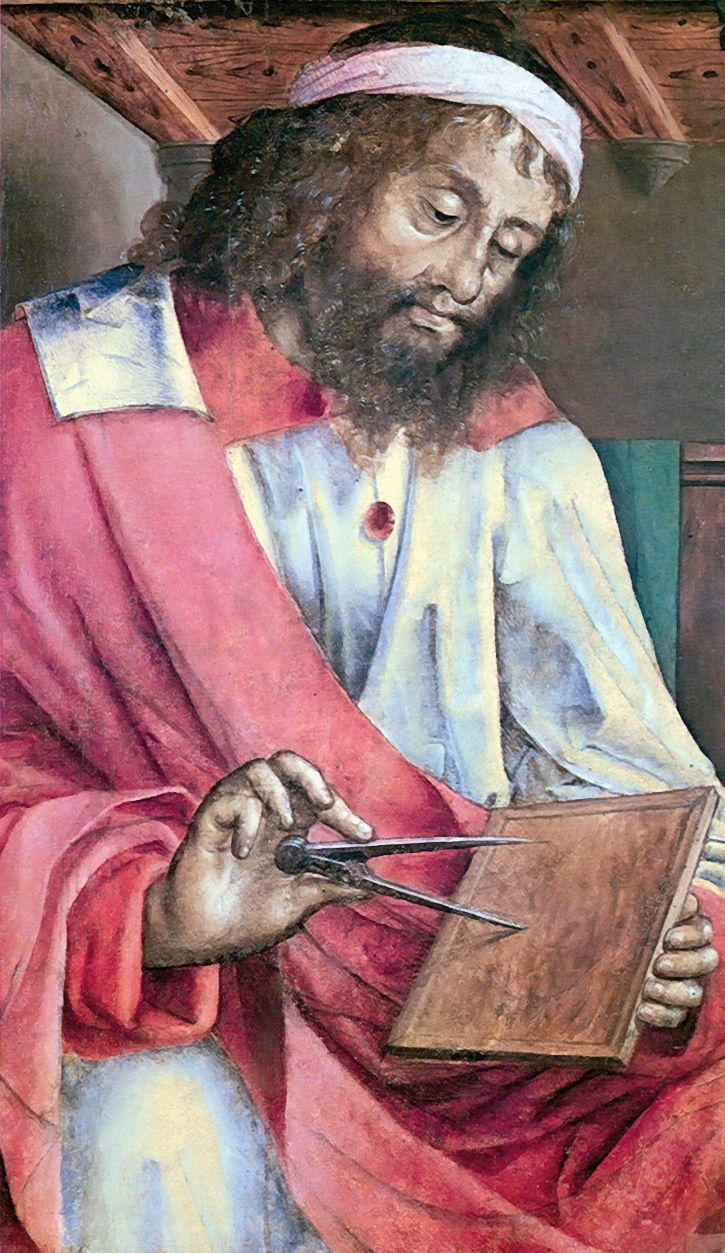
\includegraphics[scale=0.2]{figures/video_010_euklid.jpg}
\end{minipage}%
\hfill%
\begin{minipage}{0.6\textwidth}
Определение. 

\alert{Евклидова длина} или \alert{норма} вектора 

$\norm{\bx} = \sqrt{x_1^2 + x_2^2 + \ldots + x_n^2}$.
\end{minipage}

\figcaption{Евклид, около 300 лет до н.э.}

\graylink{wikipedia.org / общественное достояние}



\end{frame}



\begin{frame}
\begin{tikzpicture}[
scale=1.6,
MyPoints/.style={draw=blue,fill=white,thick},
Segments/.style={draw=blue!50!red!70,thick},
MyCircles/.style={green!50!blue!50,thin}, 
every node/.style={scale=1}
]
\grid;
\clip (-2.5,-2.5) rectangle (10.5,6.5);


%\draw[->, >=stealth] (-1,0)--(6.5,0) node[right]{$x_1$};
\draw[-{Latex[length=4.5mm, width=2.5mm]}, >=stealth] (0,-1)--(0,5) node[above left]{$x_2$};

\draw[-{Latex[length=4.5mm, width=2.5mm]}, >=stealth] (-1,0)--(6.5,0) 
node[right]{$x_1$};


%{\verb!->!new, arrowhead = 2mm, line width=4pt}
%, arrowhead = 3mm
%, arrowhead = 0.2

% Feel free to change here coordinates of points A and B
\pgfmathparse{0}		\let\Xa\pgfmathresult
\pgfmathparse{0}		\let\Ya\pgfmathresult
\coordinate (A) at (\Xa,\Ya);

\pgfmathparse{4}		\let\Xb\pgfmathresult
\pgfmathparse{3}		\let\Yb\pgfmathresult
\coordinate (B) at (\Xb,\Yb);

\pgfmathparse{4}		\let\Xc\pgfmathresult
\pgfmathparse{0}		\let\Yc\pgfmathresult
\coordinate (C) at (\Xc,\Yc);


% Let I be the midpoint of [AB]
\pgfmathparse{(\Xb+\Xa)/2} \let\XI\pgfmathresult
\pgfmathparse{(\Yb+\Ya)/2} \let\YI\pgfmathresult
\coordinate (I) at (\XI,\YI);	


\draw[-{Latex[length=4.5mm, width=2.5mm]}, >=stealth, vecb,thick] (A)--(B) node[midway,above]{$\bx$};

\draw[black, dashed, thick] (B)--(C) node[midway,right]{$3$};

\draw[black] (A)--(C) node[midway,below]{$4$};

\tkzMarkRightAngle[size=.3](A,C,B) 

\node [above right,darkgray] at (1,3.5) {$\bx=\left(\begin{array}{l}4 \\ 3\end{array}\right) \quad \|\bx\|=\sqrt{3^{2}+4^{2}}=5 $};

\end{tikzpicture}



\end{frame}




\begin{frame}{Сложение и вычитание двух векторов}

 Определение. \alert{Сложение и вычитание} двух векторов выполняем поэлементно:
    \[
    \begin{pmatrix}
      2 \\
      3.5 \\
      -1 
    \end{pmatrix} + \begin{pmatrix}
      3 \\
      -3 \\
      1 
    \end{pmatrix}  = \begin{pmatrix}
      5 \\
      0.5 \\
      0 
    \end{pmatrix}
    \]  


\begin{tikzpicture}[
scale=1.2,
MyPoints/.style={draw=blue,fill=white,thick},
Segments/.style={draw=blue!50!red!70,thick},
MyCircles/.style={green!50!blue!50,thin}, 
every node/.style={scale=1.2}
]
%\grid;
%\clip (-.5,-.5) rectangle (5.5,5.5);


%%\draw[->, >=stealth] (-1,0)--(6.5,0) node[right]{$x_1$};
%\draw[-{Latex[length=4.5mm, width=2.5mm]}, >=stealth] (0,-1)--(0,5) node[above left]{$x_2$};
%
%\draw[-{Latex[length=4.5mm, width=2.5mm]}, >=stealth] (-1,0)--(6.5,0) 
%node[right]{$x_1$};

% Feel free to change here coordinates of points A and B
\pgfmathparse{0}		\let\Xa\pgfmathresult
\pgfmathparse{0}		\let\Ya\pgfmathresult
\coordinate (A) at (\Xa,\Ya);

\pgfmathparse{2}		\let\Xb\pgfmathresult
\pgfmathparse{4}		\let\Yb\pgfmathresult
\coordinate (B) at (\Xb,\Yb);

\pgfmathparse{3}		\let\Xc\pgfmathresult
\pgfmathparse{1}		\let\Yc\pgfmathresult
\coordinate (C) at (\Xc,\Yc);

\pgfmathparse{5}		\let\Xd\pgfmathresult
\pgfmathparse{5}		\let\Yd\pgfmathresult
\coordinate (D) at (\Xd,\Yd);



% Let I be the midpoint of [AB]
\pgfmathparse{(\Xb+\Xa)/2} \let\XI\pgfmathresult
\pgfmathparse{(\Yb+\Ya)/2} \let\YI\pgfmathresult
\coordinate (I) at (\XI,\YI);	


\draw[-{Latex[length=4.5mm, width=2.5mm]}, >=stealth, vecb,thick] (A)--(B) node[midway,left]{$\ba$};

\draw[-{Latex[length=4.5mm, width=1.5mm]}, >=stealth, vecb,dashed] (C)--(D) node[midway,right]{$\ba$};


\draw[-{Latex[length=4.5mm, width=2.5mm]}, >=stealth, veca,thick] (A)--(C) node[midway,below]{$\bb$};

\draw[-{Latex[length=4.5mm, width=1.5mm]}, >=stealth, veca,dashed] (B)--(D) node[midway,above]{$\bb$};


\draw[-{Latex[length=4.5mm, width=2.5mm]}, >=stealth, vecc,thick] (A)--(D) node[midway,above, sloped]{$\ba+\bb$};


\end{tikzpicture}


\end{frame}



\begin{frame}{Умножение вектора на число}


Определение. \alert{Умножение} вектора на число выполняем поэлеметно:
    \[
    4 \cdot \begin{pmatrix}
      2 \\
      3.5 \\
      -1 
    \end{pmatrix} = \begin{pmatrix}
      8 \\
      14 \\
      -4 
    \end{pmatrix}  
    \]



\begin{tikzpicture}[
  scale=1.2,
  MyPoints/.style={draw=blue,fill=white,thick},
  Segments/.style={draw=blue!50!red!70,thick},
  MyCircles/.style={green!50!blue!50,thin}, 
  every node/.style={scale=1.2}
  ]
  %\grid;
  %\clip (-.5,-.5) rectangle (5.5,5.5);

  \pgfmathparse{0}		\let\Xa\pgfmathresult
  \pgfmathparse{0}		\let\Ya\pgfmathresult
  \coordinate (A) at (\Xa,\Ya);

  \pgfmathparse{3}		\let\Xb\pgfmathresult
  \pgfmathparse{3}		\let\Yb\pgfmathresult
  \coordinate (B) at (\Xb,\Yb);

  \pgfmathparse{5}		\let\Xc\pgfmathresult
  \pgfmathparse{5}		\let\Yc\pgfmathresult
  \coordinate (C) at (\Xc,\Yc);

  \draw[-{Latex[length=4.5mm, width=2.5mm]}, >=stealth, black,thick] (A)--(C) node[above left]{$\lambda \cdot \ba$};

  \draw[-{Latex[length=4.5mm, width=2.5mm]}, >=stealth, veca,thick] (A)--(B) node[midway,above left]{$\ba$};


  \end{tikzpicture}


\end{frame}




\begin{frame}{Расстояние между векторами}

Определение. \alert{Евклидово расстояние} между векторами
  \[
  d(\ba, \bb) = \norm{\ba - \bb} = \sqrt{(a_1 - b_1)^2 + \ldots + (a_n - b_n)^2}
  \]

\begin{itemize}
  \item по определению, $d(\ba, \bb) \geq 0$. 
  \item также говорят \alert{Евклидова метрика}
\end{itemize}


\begin{tikzpicture}[
scale=1.2,
MyPoints/.style={draw=blue,fill=white,thick},
Segments/.style={draw=blue!50!red!70,thick},
MyCircles/.style={green!50!blue!50,thin}, 
every node/.style={scale=1.2}
]
%\grid;
%\clip (-.5,-.5) rectangle (5.5,5.5);


%%\draw[->, >=stealth] (-1,0)--(6.5,0) node[right]{$x_1$};
%\draw[-{Latex[length=4.5mm, width=2.5mm]}, >=stealth] (0,-1)--(0,5) node[above left]{$x_2$};
%
%\draw[-{Latex[length=4.5mm, width=2.5mm]}, >=stealth] (-1,0)--(6.5,0) 
%node[right]{$x_1$};

% Feel free to change here coordinates of points A and B
\pgfmathparse{0}		\let\Xa\pgfmathresult
\pgfmathparse{0}		\let\Ya\pgfmathresult
\coordinate (A) at (\Xa,\Ya);

\pgfmathparse{1}		\let\Xb\pgfmathresult
\pgfmathparse{4}		\let\Yb\pgfmathresult
\coordinate (B) at (\Xb,\Yb);

\pgfmathparse{3}		\let\Xc\pgfmathresult
\pgfmathparse{1}		\let\Yc\pgfmathresult
\coordinate (C) at (\Xc,\Yc);




% Let I be the midpoint of [AB]
\pgfmathparse{(\Xb+\Xa)/2} \let\XI\pgfmathresult
\pgfmathparse{(\Yb+\Ya)/2} \let\YI\pgfmathresult
\coordinate (I) at (\XI,\YI);	


\draw[-{Latex[length=4.5mm, width=2.5mm]}, >=stealth, vecb,thick] (A)--(B) node[midway,left]{$\ba$};


\draw[-{Latex[length=4.5mm, width=2.5mm]}, >=stealth, veca,thick] (A)--(C) node[midway,below]{$\bb$};


\draw[-{Latex[length=4.5mm, width=2.5mm]}, >=stealth, vecc,thick] (C)--(B) node[midway,right]{$\ba-\bb$};


\end{tikzpicture}
    


\end{frame}






\begin{frame}{Скалярное произведение и угол}

\begin{itemize}[<+->]
\item Определение. \alert{Скалярное произведение} векторов $\ba$ и $\bb$:
  $\langle \ba, \bb \rangle = a_1 b_1 + a_2 b_2 + \ldots + a_n b_n$.

\item Определение. 
\alert{Косинус угла} и \alert{угол} между векторами $\ba$ и $\bb$:
% Косинусная близость, cosine similarity:  
  \[
  \cos \angle (\ba, \bb) =  \frac{\langle \ba, \bb \rangle}{ \norm{\ba} \norm{\bb}} \quad   \angle (\ba, \bb) =  \arccos \frac{\langle \ba, \bb \rangle}{ \norm{\ba} \norm{\bb}} 
  \]
\end{itemize}

\begin{tikzpicture}[
scale=1.2,
MyPoints/.style={draw=blue,fill=white,thick},
Segments/.style={draw=blue!50!red!70,thick},
MyCircles/.style={green!50!blue!50,thin}, 
every node/.style={scale=1.2}
]
%\grid;

%\clip (-.5,-.5) rectangle (6.5,5.5);


%%\draw[->, >=stealth] (-1,0)--(6.5,0) node[right]{$x_1$};
%\draw[-{Latex[length=4.5mm, width=2.5mm]}, >=stealth] (0,-1)--(0,5) node[above left]{$x_2$};
%
%\draw[-{Latex[length=4.5mm, width=2.5mm]}, >=stealth] (-1,0)--(6.5,0) 
%node[right]{$x_1$};

% Feel free to change here coordinates of points A and B
\pgfmathparse{0}		\let\Xa\pgfmathresult
\pgfmathparse{0}		\let\Ya\pgfmathresult
\coordinate (A) at (\Xa,\Ya);

\pgfmathparse{1}		\let\Xb\pgfmathresult
\pgfmathparse{4}		\let\Yb\pgfmathresult
\coordinate (B) at (\Xb,\Yb);

\pgfmathparse{4}		\let\Xc\pgfmathresult
\pgfmathparse{1}		\let\Yc\pgfmathresult
\coordinate (C) at (\Xc,\Yc);


\draw[-{Latex[length=4.5mm, width=2.5mm]}, >=stealth, vecb,thick] (A)--(B) node[midway,left]{$\ba$};


\draw[-{Latex[length=4.5mm, width=2.5mm]}, >=stealth, veca,thick] (A)--(C) node[midway,below]{$\bb$};


\tkzMarkAngle[size=1, mark = none](C,A,B);

\node [darkgray] at (1,1) {$\varphi$}; 

% \node [above right, darkgray] at (2, 2) {$\cos \varphi=\dfrac{\langle \ba, \bb\rangle}{\|\ba\| \cdot\|\bb\|}$}; 

%\draw
%(3,-1) coordinate (a) node[right] {$a$}
%-- (0,0) coordinate (b) node[left] {b}
%-- (2,2) coordinate (c) node[above right] {c}


\end{tikzpicture}
  
Угол определён, если $\norm{\ba} > 0$ и $\norm{\bb} > 0$.


\end{frame}



\begin{frame}{Скалярное произведение и проекция}

  Если вектор $\ba$ имеет единичную длину, $\norm{\ba} = 1$, то 


  $\langle \ba, \bb \rangle = \norm{\bb} \cos \phi$ — длина$^*$ проекции $b$ на $a$.
  

\begin{tikzpicture}[
scale=1.2,
MyPoints/.style={draw=blue,fill=white,thick},
Segments/.style={draw=blue!50!red!70,thick},
MyCircles/.style={green!50!blue!50,thin}, 
every node/.style={scale=1.2}
]
%\grid;

%\clip (-1.5,-1.5) rectangle (7.5,5.5);


%%\draw[->, >=stealth] (-1,0)--(6.5,0) node[right]{$x_1$};
%\draw[-{Latex[length=4.5mm, width=2.5mm]}, >=stealth] (0,-1)--(0,5) node[above left]{$x_2$};
%
%\draw[-{Latex[length=4.5mm, width=2.5mm]}, >=stealth] (-1,0)--(6.5,0) 
%node[right]{$x_1$};

% Feel free to change here coordinates of points A and B
\pgfmathparse{0}		\let\Xa\pgfmathresult
\pgfmathparse{0}		\let\Ya\pgfmathresult
\coordinate (A) at (\Xa,\Ya);

\pgfmathparse{5.5}		\let\Xb\pgfmathresult
\pgfmathparse{5.5}		\let\Yb\pgfmathresult
\coordinate (B) at (\Xb,\Yb);

\pgfmathparse{5}		\let\Xc\pgfmathresult
\pgfmathparse{2}		\let\Yc\pgfmathresult
\coordinate (C) at (\Xc,\Yc);

\pgfmathparse{-1}		\let\Xd\pgfmathresult
\pgfmathparse{1}		\let\Yd\pgfmathresult
\coordinate (D) at (\Xd,\Yd);

\pgfmathparse{3}		\let\Xe\pgfmathresult
\pgfmathparse{5}		\let\Ye\pgfmathresult
\coordinate (E) at (\Xe,\Ye);

\pgfmathparse{-0.75}		\let\Xf\pgfmathresult
\pgfmathparse{0.75}		\let\Yf\pgfmathresult
\coordinate (F) at (\Xf,\Yf);

\pgfmathparse{3.25}		\let\Xg\pgfmathresult
\pgfmathparse{4.75}		\let\Yg\pgfmathresult
\coordinate (G) at (\Xg,\Yg);

\pgfmathparse{4}		\let\Xh\pgfmathresult
\pgfmathparse{4}		\let\Yh\pgfmathresult
\coordinate (H) at (\Xh,\Yh);

\pgfmathparse{6}		\let\Xj\pgfmathresult
\pgfmathparse{2}		\let\Yj\pgfmathresult
\coordinate (J) at (\Xj,\Yj);

\draw[-{Latex[length=4.5mm, width=2.5mm]}, >=stealth, vecb,thick] (A)--(B) node[midway,left]{$\ba$};


\draw[-{Latex[length=4.5mm, width=2.5mm]}, >=stealth, veca,thick] (A)--(J) node[midway,below]{$\bb$};

\draw[thick] (A)--(D);
\draw[thick] (H)--(E);

\draw[thick, dashed] (J)--(E);


\draw[{Latex[length=4.5mm, width=2.5mm]}-{Latex[length=4.5mm, width=2.5mm]}, >=stealth, thick] (F)--(G) node[midway,above left]{$\langle \ba, \bb \rangle$};




\tkzMarkRightAngle[size=0.3, mark = none](A,H,J);

\tkzMarkAngle[size=1, mark = none](C,A,B);


%\node [below, darkgray] at (1,1) {$\varphi$}; 

%\node [below right, darkgray] at (-1.5,-1) {если  $\| \ba \| = 1 $, то $\langle \ba, \bb \rangle$  -- длина* проекции $\bb$ на $\ba$}; 



%\draw
%(3,-1) coordinate (a) node[right] {$a$}
%-- (0,0) coordinate (b) node[left] {b}
%-- (2,2) coordinate (c) node[above right] {c}


\end{tikzpicture}




\end{frame}


\begin{frame}{Свойства скалярного произведения}

  
  \begin{itemize}[<+->]
  \item Скалярное вектора на себя равно квадрату длины
  $\langle \ba, \ba \rangle = \norm{\ba}^2$

  \item Линейность по каждому аргументу
  $\langle \lambda \ba, \bb \rangle = \langle \ba,  \lambda  \bb \rangle = \lambda  \langle \ba,  \bb \rangle$

  $\langle \ba + \bb, \bc \rangle = \langle \ba , \bc \rangle + \langle \bb , \bc \rangle$

  \item Симметричность
  
  $\langle \ba, \bb \rangle = \langle \bb, \ba \rangle$
  \end{itemize}
  
  

\end{frame}





% \begin{frame}{Почти любой объект — вектор!}

%   \begin{block}{С помощью вектора можно закодировать:}
%   \begin{itemize}
%     \item многочлен 
%     \[
%     3x^2 + 6 x - 7 \to (3, 6, -7)  
%     \]
%     \item характеристики индивида

%     \[
%     \text{Блондин с ростом 182 см и весов 81 килограмм} \to (0, 182, 81)
%     \]
%     \item TODO
%   \end{itemize}

%   \end{block}
% \end{frame}




\begin{frame}{Ортогональность векторов}

Определение. Векторы $\ba$ и $\bb$ \alert{ортогональны}, $a\perp b$, если
\[
  \langle \ba, \bb \rangle =0
\]

Также говорят «\alert{перпендикулярны}».


\begin{tikzpicture}[
scale=1.8,
MyPoints/.style={draw=blue,fill=white,thick},
Segments/.style={draw=blue!50!red!70,thick},
MyCircles/.style={green!50!blue!50,thin}, 
every node/.style={scale=1.2}
]
%\grid;

\clip (-1.5,-1.5) rectangle (8.5,5.5);


%%\draw[->, >=stealth] (-1,0)--(6.5,0) node[right]{$x_1$};
%\draw[-{Latex[length=4.5mm, width=2.5mm]}, >=stealth] (0,-1)--(0,5) node[above left]{$x_2$};
%
%\draw[-{Latex[length=4.5mm, width=2.5mm]}, >=stealth] (-1,0)--(6.5,0) 
%node[right]{$x_1$};

% Feel free to change here coordinates of points A and B
\pgfmathparse{0}		\let\Xa\pgfmathresult
\pgfmathparse{0}		\let\Ya\pgfmathresult
\coordinate (A) at (\Xa,\Ya);

\pgfmathparse{1}		\let\Xb\pgfmathresult
\pgfmathparse{4}		\let\Yb\pgfmathresult
\coordinate (B) at (\Xb,\Yb);

\pgfmathparse{4}		\let\Xc\pgfmathresult
\pgfmathparse{-1}		\let\Yc\pgfmathresult
\coordinate (C) at (\Xc,\Yc);

\pgfmathparse{-1}		\let\Xc\pgfmathresult
\pgfmathparse{4}		\let\Yc\pgfmathresult
\coordinate (D) at (\Xc,\Yc);



\draw[-{Latex[length=4.5mm, width=2.5mm]}, >=stealth, vecb,thick] (A)--(B) node[above left]{$\ba$};


\draw[-{Latex[length=4.5mm, width=2.5mm]}, >=stealth, veca,thick] (A)--(C) node[above right]{$\bb$};

\draw[-{Latex[length=4.5mm, width=2.5mm]}, >=stealth, thick] (A)--(D) node[above left]{$\bc$};


\tkzMarkRightAngle[size=0.5](C,A,B);


\node [above right, darkgray] at (2, 2) {$\begin{array}{l}
  \ba \perp \bb \text{ так как } \langle \ba, \bb \rangle =0 \\
  \ba \nperp \bc  \text{ так как } 
  \langle \ba, \bc \rangle  \neq 0
  \end{array}$}; 



%\draw
%(3,-1) coordinate (a) node[right] {$a$}
%-- (0,0) coordinate (b) node[left] {b}
%-- (2,2) coordinate (c) node[above right] {c}


\end{tikzpicture}


\end{frame}



    


% % !TEX root = ../linal_lecture_01.tex

\begin{frame} % название фрагмента

\videotitle{Прямая, порожденная вектором, гиперплоскость} % Порожденные вектором

\end{frame}


\begin{frame}{Краткий план:}

\begin{itemize}[<+->]
  \item Да будет больше разных расстояний!
  \item Делаем из вектора прямую.
  \item Делаем из вектора гиперплоскость.
  % Ядерные функции из скалярного произведения. - в упражнения!
\end{itemize}

\end{frame}


\begin{frame}{Больше метрик в студию!}

 \begin{block}{Определение} 
 \alert{Манхэттэнская метрика} или \alert{расстояние по-Майкопски}:
  \[
  d(\ba, \bb) = \abs{a_1 - b_1}  + \abs{a_2 - b_2} + \ldots + \abs{a_n - b_n}
  \]
 \end{block}

\end{frame}




\begin{frame}{У них — Манхэттэн}
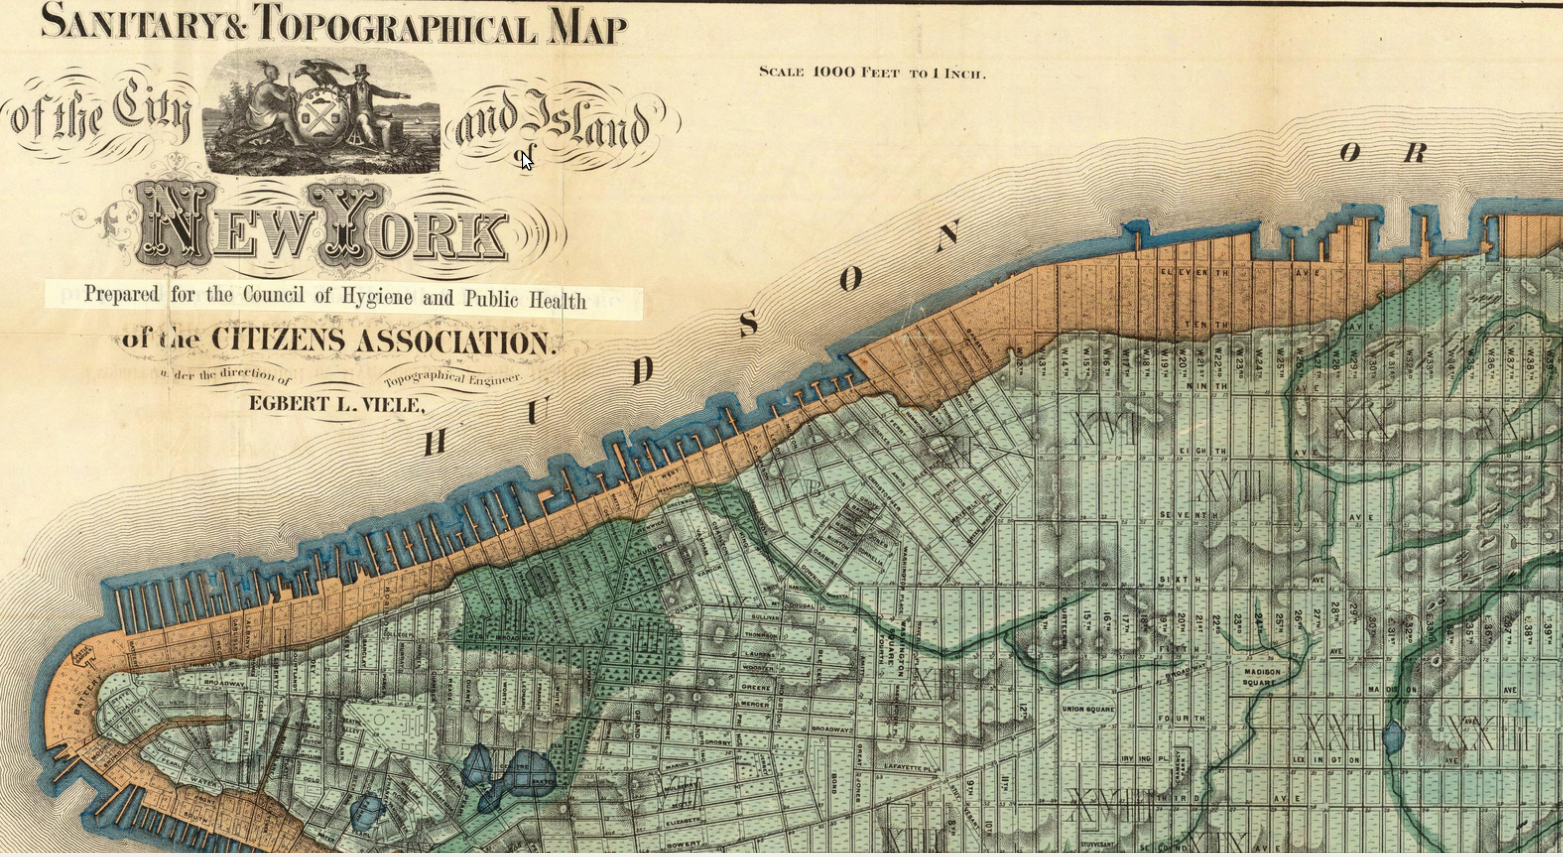
\includegraphics[scale=0.5]{figures/video_010_manhattan.png}

% \figcaption{План Манхэттэна}

\graylink{wikipedia.org / общественное достояние}
\end{frame}



\begin{frame}{У нас — Майкоп}
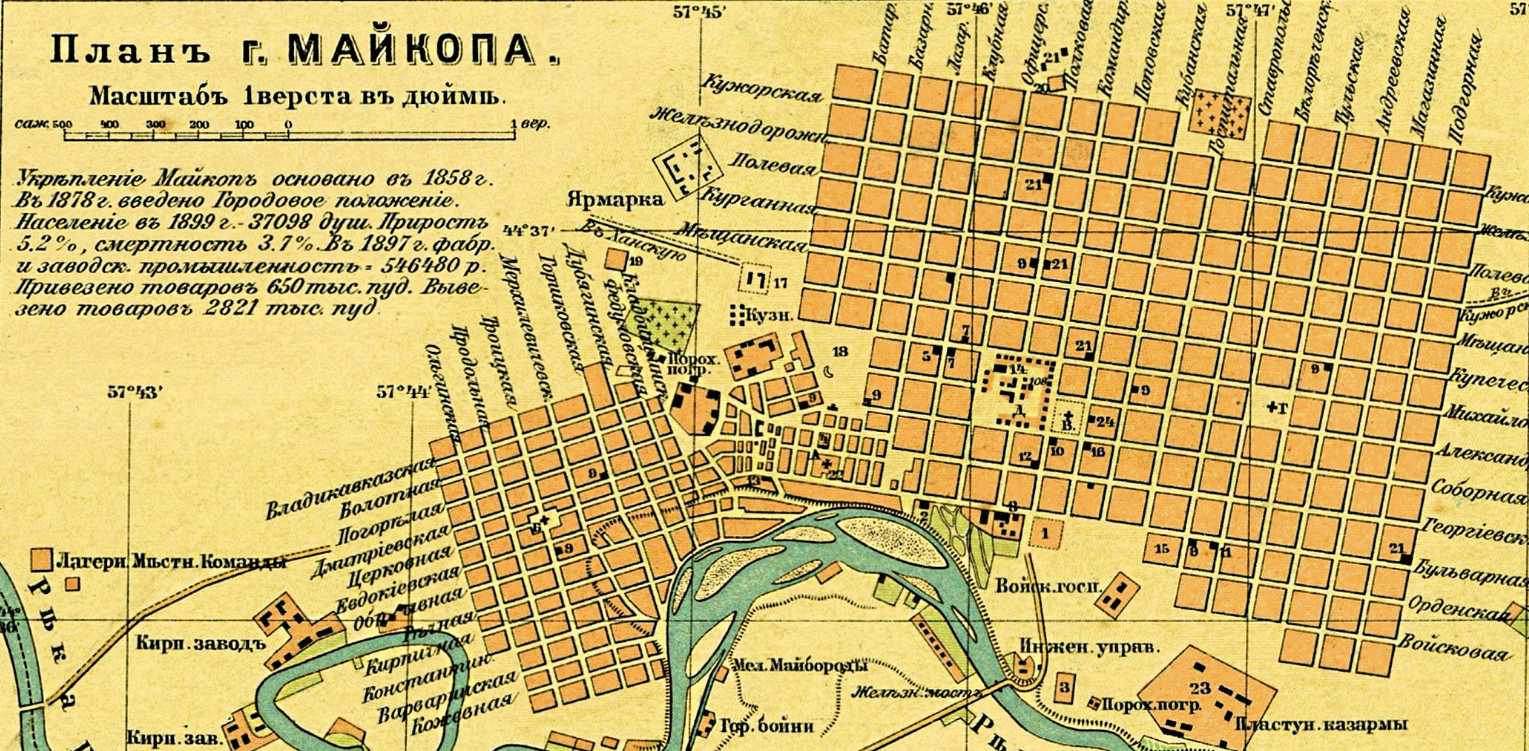
\includegraphics[scale=0.5]{figures/video_010_maykop.png}

% \figcaption{План Майкопа}

\graylink{wikipedia.org / общественное достояние}
    

\end{frame}





\begin{frame}{Ещё больше метрик!}
%\begin{block}{Метрика Чебышёва}
%  \[
%      d(a, b) = \max\left\{\abs{a_1 - b_1}, \abs{a_2 - b_2}, \ldots, \abs{a_n - b_n}\right\}
%  \]
%\end{block}

\begin{block}{Определение} 

\alert{Метрика Минковского}
  \[
      d_p(\ba, \bb) = \left(\sum_{i=1}^n \abs{a_i - b_i}^p \right)^{1/p}
  \]
\end{block}
\end{frame}

\begin{frame}{Частные случаи метрики Минковского}

  
\alert{Евклидова метрика, $p=2$}
$
   d_2(\ba, \bb) = \sqrt{(a_1 - b_1)^2 + \ldots + (a_n - b_n)^2} 
$

\alert{Манхэттэнская метрика, $p=1$}
$
d_1(\ba, \bb) = \abs{a_1 - b_1}  + \abs{a_2 - b_2} + \ldots + \abs{a_n - b_n} 
$

%\begin{block}{Метрика Чебышёва, $p\to \infty$}
%$
    %\max\left\{\abs{a_1 - b_1}, \ldots, \abs{a_n - b_n}\right\} = \lim_{p\to\infty} d_p(a, b)
%$
%\end{block}

\begin{tikzpicture}[
scale=1.8,
MyPoints/.style={draw=blue,fill=white,thick},
Segments/.style={draw=blue!50!red!70,thick},
MyCircles/.style={green!50!blue!50,thin}, 
every node/.style={scale=1.2}
]

\draw[color=gray,step=1.0,dotted] (-1.1,-2.1) grid (7.6,6.1);
%\grid;


%%\draw[->, >=stealth] (-1,0)--(6.5,0) node[right]{$x_1$};
%\draw[-{Latex[length=4.5mm, width=2.5mm]}, >=stealth] (0,-1)--(0,5) node[above left]{$x_2$};
%
%\draw[-{Latex[length=4.5mm, width=2.5mm]}, >=stealth] (-1,0)--(6.5,0) 
%node[right]{$x_1$};

% Feel free to change here coordinates of points A and B
\pgfmathparse{0}		\let\Xa\pgfmathresult
\pgfmathparse{0}		\let\Ya\pgfmathresult
\coordinate (A) at (\Xa,\Ya);

\pgfmathparse{1}		\let\Xb\pgfmathresult
\pgfmathparse{4}		\let\Yb\pgfmathresult
\coordinate (B) at (\Xb,\Yb);

\pgfmathparse{5}		\let\Xc\pgfmathresult
\pgfmathparse{1}		\let\Yc\pgfmathresult
\coordinate (C) at (\Xc,\Yc);

\pgfmathparse{5}		\let\Xd\pgfmathresult
\pgfmathparse{4}		\let\Yd\pgfmathresult
\coordinate (D) at (\Xd,\Yd);




% Let I be the midpoint of [AB]
\pgfmathparse{(\Xb+\Xa)/2} \let\XI\pgfmathresult
\pgfmathparse{(\Yb+\Ya)/2} \let\YI\pgfmathresult
\coordinate (I) at (\XI,\YI);	


\draw[-{Latex[length=4.5mm, width=2.5mm]}, >=stealth, darkgray,thick] (A)--(B) node[midway,left]{$\ba$};


\draw[-{Latex[length=4.5mm, width=2.5mm]}, >=stealth, darkgray,thick] (A)--(C) node[midway,below]{$\bb$};

\draw[veca,thick, line width=0.35mm] (D)--(B);
\draw[veca,thick, line width=0.35mm] (C)--(D);


\draw[vecb,thick, line width=0.35mm] (C)--(B) node[midway,below left ]{$d_2(\ba,\bb)$};

\draw[vecc,thick, line width=0.35mm] (C) to[bend right] (B);

\node [above, vecc] at (4,3) {$d_p(\ba,\bb)$};



\node [above right, veca] at (4, 4) {$d_1(\ba,\bb)$}; 

\end{tikzpicture}

    


\end{frame}





\begin{frame}{Вектор порождает прямую}

\begin{block}{Определение} 
\alert{Прямая порождённая вектором $a$}, $\Span a$

Множество векторов, получаемых при домножении вектора $a$ на произвольное число,
\[
\Span \ba = \left\{t\cdot \ba \middle| t \in \R \right\}  
\]
\end{block}

\pause

\begin{tikzpicture}[
scale=1.2,
MyPoints/.style={draw=blue,fill=white,thick},
Segments/.style={draw=blue!50!red!70,thick},
MyCircles/.style={green!50!blue!50,thin}, 
every node/.style={scale=1.2}
]
%\grid;
\clip (-1.5,-1.5) rectangle (5.5,5.5);

\pgfmathparse{1}		\let\Xa\pgfmathresult
\pgfmathparse{1}		\let\Ya\pgfmathresult
\coordinate (A) at (\Xa,\Ya);

\pgfmathparse{3}		\let\Xb\pgfmathresult
\pgfmathparse{3}		\let\Yb\pgfmathresult
\coordinate (B) at (\Xb,\Yb);

\pgfmathparse{5}		\let\Xc\pgfmathresult
\pgfmathparse{5}		\let\Yc\pgfmathresult
\coordinate (C) at (\Xc,\Yc);

\pgfmathparse{-1}		\let\Xd\pgfmathresult
\pgfmathparse{-1}		\let\Yd\pgfmathresult
\coordinate (D) at (\Xd,\Yd);



\draw[ black,dashed] (D)--(C); % node[above left]{$\Span \ba$};

\draw[-{Latex[length=4.5mm, width=2.5mm]}, >=stealth, veca,thick] (A)--(B) node[midway,above left]{$\ba$};


\end{tikzpicture}


\end{frame}





\begin{frame}{Вектор задаёт гиперплоскость}

Вектор $\ba$ фиксирован, например, $\ba=(1, 2)$.

%\begin{block}{TODO: две картинки рядом}
%$\langle \ba, \bv \rangle = 0$ и $\langle \ba, \bv \rangle = 1$   
%\end{block}


\begin{minipage}{0.45\textwidth}
    
\begin{tikzpicture}[
scale=1.2,
MyPoints/.style={draw=blue,fill=white,thick},
Segments/.style={draw=blue!50!red!70,thick},
MyCircles/.style={green!50!blue!50,thin}, 
every node/.style={scale=1.2}
]
%\grid;
\clip (-1.5,-1.5) rectangle (5.5,6.5);

\pgfmathparse{2}		\let\Xa\pgfmathresult
\pgfmathparse{2}		\let\Ya\pgfmathresult
\coordinate (A) at (\Xa,\Ya);

\pgfmathparse{4}		\let\Xb\pgfmathresult
\pgfmathparse{4}		\let\Yb\pgfmathresult
\coordinate (B) at (\Xb,\Yb);

\pgfmathparse{-1}		\let\Xc\pgfmathresult
\pgfmathparse{5}		\let\Yc\pgfmathresult
\coordinate (C) at (\Xc,\Yc);

\pgfmathparse{5}		\let\Xd\pgfmathresult
\pgfmathparse{-1}		\let\Yd\pgfmathresult
\coordinate (D) at (\Xd,\Yd);

\pgfmathparse{0}		\let\Xe\pgfmathresult
\pgfmathparse{4}		\let\Ye\pgfmathresult
\coordinate (E) at (\Xe,\Ye);



\draw[ black,dashed] (D)--(C);

\draw[-{Latex[length=4.5mm, width=2.5mm]}, >=stealth, veca,thick] (A)--(B) node[midway,above left]{$\ba$};

\draw[-{Latex[length=4.5mm, width=2.5mm]}, >=stealth, vecb,thick] (A)--(E) node[midway,below left]{$\bv$};

\tkzMarkRightAngle[size=0.3](E,A,B);


\node [above right] at (1, 4.5) {$\langle \ba, \bv  \rangle = 0$}; 


\end{tikzpicture}
\end{minipage}
\hfill
\begin{minipage}{0.45\textwidth}
\begin{tikzpicture}[
scale=1.2,
MyPoints/.style={draw=black,fill=red,thick},
Segments/.style={draw=blue!50!red!70,thick},
MyCircles/.style={green!50!blue!50,thin}, 
every node/.style={scale=1.2}
]
%\grid;
\clip (-1.5,-1.5) rectangle (5.5,6.5);

\pgfmathparse{0}		\let\Xa\pgfmathresult
\pgfmathparse{0}		\let\Ya\pgfmathresult
\coordinate (A) at (\Xa,\Ya);

\pgfmathparse{3}		\let\Xb\pgfmathresult
\pgfmathparse{3}		\let\Yb\pgfmathresult
\coordinate (B) at (\Xb,\Yb);

\pgfmathparse{-1}		\let\Xc\pgfmathresult
\pgfmathparse{5}		\let\Yc\pgfmathresult
\coordinate (C) at (\Xc,\Yc);

\pgfmathparse{5}		\let\Xd\pgfmathresult
\pgfmathparse{-1}		\let\Yd\pgfmathresult
\coordinate (D) at (\Xd,\Yd);

\pgfmathparse{0}		\let\Xe\pgfmathresult
\pgfmathparse{4}		\let\Ye\pgfmathresult
\coordinate (E) at (\Xe,\Ye);

\pgfmathparse{2}		\let\Xf\pgfmathresult
\pgfmathparse{2}		\let\Yf\pgfmathresult
\coordinate (F) at (\Xf,\Yf);



\draw[ black,dashed] (D)--(C);

\draw[-{Latex[length=4.5mm, width=2.5mm]}, >=stealth, veca,thick] (A)--(B) node[below right]{$\ba$};

\draw[-{Latex[length=4.5mm, width=2.5mm]}, >=stealth, vecb,thick] (A)--(E) node[below left]{$\bv$};

\draw[veca,thick] (A)--(F) node[midway,below right]{$\frac{1}{\|\ba\|}$};



\node [above right] at (1, 4.5) {$\langle \ba, \bv  \rangle = 1$}; 

\node [below left] at (A) {$0$}; 


\fill[MyPoints] (A) circle (0.8mm);
\fill[MyPoints] (F) circle (0.8mm);


\end{tikzpicture}


\end{minipage}


$a_1 v_1 + a_2 v_2 = 0$ \hspace{8cm} $a_1 v_1 + a_2 v_2 = 1$

\end{frame}



% \begin{frame}{Ядерные функции}

% Векторная функция $f$ фиксирована, например, 
% \[
%   f : \begin{pmatrix}
%     v_1 \\
%     v_2 \\
%   \end{pmatrix} \to 
%   \begin{pmatrix}
%     -1 \\
%     v_1^2 + v_2^2 \\
%   \end{pmatrix}
% \]

% \begin{block}{Ядерная функция, ядро $K$}
% Скалярное произведение в спрямляющем пространстве:
% $K(a, b) = \langle f(a), f(b) \rangle$.
% \end{block}
% \end{frame}

% \begin{frame}
%   \frametitle{Спрямляющее пространство:}

% \begin{block}{TODO: картинка с исходным и спрямляющим пространством} 

% \end{block}


% \end{frame}

    



  
% % !TEX root = ../linal_lecture_01.tex


\begin{frame} % название фрагмента

\videotitle{Линейный оператор: определение и примеры}

% примеры: R^n -> R^n: перестановка координат, растягивание, проекция, поворот, единичный оператор
% R^n -> R^k: обрезка, дописывание нулей,

\end{frame}


\begin{frame}{Краткий план:}

\begin{itemize}[<+->]
  \item Определение линейного оператора.
  \item Примеры линейных операторов.
  \item Как из двух операторов сделать новый оператор?
  % Ядерные функции из скалярного произведения. - в упражнения!
\end{itemize}

\end{frame}
    


\begin{frame}{Линейный оператор}


\alert{Идея линейности}:
  
Результат действия $\LL$ не изменится, 

если поменять местами действие $\LL$ и

\begin{itemize}[<+->]
    \item растягивание вектора, например, $\LL(42a)=42\LL(a)$;
    \item усреднение двух векторов, $\LL(0.5a+0.5b)=0.5\LL(a) + 0.5\LL(b)$.
  \end{itemize}


\end{frame}


\begin{frame}{Стандартное определение линейности}

\begin{block}{Определение}
Функция $\LL$, превращающая векторы из $\R^n$ в векторы $\R^k$, называется 
\alert{линейным оператором} если:

\begin{itemize}[<+->]
  \item для любого числа $t$ и вектора $a \in \R^n$: $\LL(t a) = t\LL(a)$;
  \item для любых двух векторов $a$ и $b$ из $\R^n$: $\LL(a + b) = \LL(a) + \LL(b)$. 
\end{itemize}
\end{block}

\pause
\vspace{10pt}
Вместо скобок часто пишут знак умножения, 

$\LL(a) \equiv \LL \cdot a \equiv \LL a$.

\end{frame}


\begin{frame}{Линейный оператор}

\begin{center}
\begin{tikzpicture}[
scale=2,
MyPoints/.style={draw=blue,fill=white,thick},
Segments/.style={draw=blue!50!red!70,thick},
MyCircles/.style={green!50!blue!50,thin}, 
every node/.style={scale=1}
]
\draw[color=gray,step=1.0,dotted] (-1.9,-0.9) grid (7.5,7.0); 
% \clip (-1.5,-0.5) rectangle (6.1,6.5);

%{\verb!->!new, arrowhead = 2mm, line width=4pt}
%, arrowhead = 3mm
%, arrowhead = 0.2

% Feel free to change here coordinates of points A and B
\pgfmathparse{0}		\let\Xa\pgfmathresult
\pgfmathparse{4}		\let\Ya\pgfmathresult
\coordinate (A) at (\Xa,\Ya);

\pgfmathparse{0}		\let\Xb\pgfmathresult
\pgfmathparse{5}		\let\Yb\pgfmathresult
\coordinate (B) at (\Xb,\Yb);

\pgfmathparse{2}		\let\Xc\pgfmathresult
\pgfmathparse{5}		\let\Yc\pgfmathresult
\coordinate (C) at (\Xc,\Yc);

\pgfmathparse{2}		\let\Xd\pgfmathresult
\pgfmathparse{4}		\let\Yd\pgfmathresult
\coordinate (D) at (\Xd,\Yd);

\pgfmathparse{4}		\let\Xe\pgfmathresult
\pgfmathparse{4}		\let\Ye\pgfmathresult
\coordinate (E) at (\Xe,\Ye);

\pgfmathparse{0}		\let\Xf\pgfmathresult
\pgfmathparse{1}		\let\Yf\pgfmathresult
\coordinate (F) at (\Xf,\Yf);

\pgfmathparse{4}		\let\Xg\pgfmathresult
\pgfmathparse{1}		\let\Yg\pgfmathresult
\coordinate (G) at (\Xg,\Yg);


% Let I be the midpoint of [AB]
\pgfmathparse{(\Xb+\Xa)/2} \let\XI\pgfmathresult
\pgfmathparse{(\Yb+\Ya)/2} \let\YI\pgfmathresult
\coordinate (I) at (\XI,\YI);	


\draw[-{Latex[length=4.5mm, width=2.5mm]}, >=stealth, veca,thick] (A)--(B) node[left]{$\left(\begin{array}{l}0 \\ 1\end{array}\right)$} ;

\draw[black, dashed, thick] (B)--(C);
\draw[black, dashed, thick] (D)--(C);
\draw[black, dashed, thick] (F)--(G);
\draw[black, dashed, thick] (E)--(G);


\draw[-{Latex[length=4.5mm, width=2.5mm]}, >=stealth,  veca] (A)--(C) node[above right]{$\ba = \begin{pmatrix} 2 \\ 1 \end{pmatrix}$};

\draw[-{Latex[length=4.5mm, width=2.5mm]}, >=stealth,  vecb] (A)--(E) node[below]{$\LL  \cdot \left(\begin{array}{l}2 \\ 0\end{array}\right)$};

\draw[-{Latex[length=4.5mm, width=2.5mm]}, >=stealth,  veca] (A)--(D) node[below]{$\left(\begin{array}{l}2 \\ 0\end{array}\right)$};

\draw[-{Latex[length=4.5mm, width=2.5mm]}, >=stealth,  vecb] (A)--(G) node[below left,pos=1.1]{$\LL  \cdot \ba $};

\draw[-{Latex[length=4.5mm, width=2.5mm]}, >=stealth,  vecb] (A)--(F) node[below]{$\LL  \cdot \left(\begin{array}{l}0 \\ 1\end{array}\right)$ };


\end{tikzpicture}
\end{center}



\end{frame}


\begin{frame}{Растягивание координат}

Обобщаем умножение вектора на число!

  $\LL : \begin{pmatrix}
    a_1 \\
    a_2 \\
  \end{pmatrix} \to 
  \begin{pmatrix}
    2a_1 \\
    -3a_2 \\
  \end{pmatrix}$


\end{frame}



\begin{frame}{Перестановка координат вектора}


$\LL : \begin{pmatrix}
    a_1 \\
    a_2 \\
    a_3 \\
  \end{pmatrix} \to 
  \begin{pmatrix}
    a_2 \\
    a_3 \\
    a_1 \\
  \end{pmatrix}$

\vspace{10pt}

Пример. \alert{Отражение относительно $x_1=x_2$}:


\begin{center}
\begin{tikzpicture}[
scale=1.8,
MyPoints/.style={draw=black,fill=black,thick},
Segments/.style={draw=blue!50!red!70,thick},
MyCircles/.style={green!50!blue!50,thin}, 
every node/.style={scale=1.2}
]
\draw[color=gray,step=1.0,dotted] (-1.5,-1.5) grid (3.5,3.5); 
% \clip (-1.5,-3.5) rectangle (3.5,3.5);

\pgfmathparse{0}		\let\Xa\pgfmathresult
\pgfmathparse{0}		\let\Ya\pgfmathresult
\coordinate (A) at (\Xa,\Ya);

\pgfmathparse{2}		\let\Xb\pgfmathresult
\pgfmathparse{1}		\let\Yb\pgfmathresult
\coordinate (B) at (\Xb,\Yb);

\pgfmathparse{3}		\let\Xc\pgfmathresult
\pgfmathparse{3}		\let\Yc\pgfmathresult
\coordinate (C) at (\Xc,\Yc);

\pgfmathparse{-1}		\let\Xd\pgfmathresult
\pgfmathparse{-1}		\let\Yd\pgfmathresult
\coordinate (D) at (\Xd,\Yd);

\pgfmathparse{1}		\let\Xe\pgfmathresult
\pgfmathparse{2}		\let\Ye\pgfmathresult
\coordinate (E) at (\Xe,\Ye);



\draw[ black,dashed] (D)--(C);

\draw[-{Latex[length=4.5mm, width=2.5mm]}, >=stealth, veca,thick] (A)--(B) node[below right]{$\left(\begin{array}{l}2 \\ 1\end{array}\right)$};

\draw[-{Latex[length=4.5mm, width=2.5mm]}, >=stealth, vecb,thick] (A)--(E) node[above left]{$\LL  \cdot \left(\begin{array}{l}2 \\ 1\end{array}\right) = \begin{pmatrix} 1 \\ 2 \end{pmatrix}$ };

% \node [right,darkgray] at (-1,-2.5) {$L:\left(\begin{array}{l}a_{1} \\ a_{2}\end{array}\right) \rightarrow\left(\begin{array}{l}a_{2} \\ a_{1}\end{array}\right)$ }; 


\fill[MyPoints]  (0,0) circle (0.8mm) node [below] {$0$};


\end{tikzpicture}
\end{center}

\end{frame}



\begin{frame}{Первый поворот}

\alert{Поворот} на $30^{\circ}$ против часовой стрелки.

Оператор $\Rot: \R^2 \to \R^2$.

\begin{center}
\begin{tikzpicture}[
scale=1.4,
MyPoints/.style={draw=blue,fill=white,thick},
Segments/.style={draw=blue!50!red!70,thick},
MyCircles/.style={blue!50,dashed}, 
every node/.style={scale=1.2}
]
%\grid;
%\draw[color=gray,step=1.0,dotted] (-7.1,-2.1) grid (7.6,6.1);
%\clip (-5.5,-.5) rectangle (5.5,5.5);


%%\draw[->, >=stealth] (-1,0)--(6.5,0) node[right]{$x_1$};
%\draw[-{Latex[length=4.5mm, width=2.5mm]}, >=stealth] (0,-1)--(0,5) node[above left]{$x_2$};
%
%\draw[-{Latex[length=4.5mm, width=2.5mm]}, >=stealth] (-1,0)--(6.5,0) 
%node[right]{$x_1$};

% Feel free to change here coordinates of points A and B
\pgfmathparse{0}		\let\Xa\pgfmathresult
\pgfmathparse{0}		\let\Ya\pgfmathresult
\coordinate (A) at (\Xa,\Ya);

\pgfmathparse{1}		\let\Xb\pgfmathresult
\pgfmathparse{3}		\let\Yb\pgfmathresult
\coordinate (B) at (\Xb,\Yb);

\pgfmathparse{3}		\let\Xc\pgfmathresult
\pgfmathparse{1}		\let\Yc\pgfmathresult
\coordinate (C) at (\Xc,\Yc);

\pgfmathparse{3}		\let\Xd\pgfmathresult
\pgfmathparse{4}		\let\Yd\pgfmathresult
\coordinate (D) at (\Xd,\Yd);

\pgfmathparse{75}		\let\angle\pgfmathresult;
\pgfmathparse{sqrt(10)}		\let\rad\pgfmathresult;


\pgfmathparse{\Xb*cos(\angle)  - \Yb*sin(\angle)}		\let\Xe\pgfmathresult
\pgfmathparse{\Xb*sin(\angle)  + \Yb*cos(\angle)}		\let\Ye\pgfmathresult
\coordinate (E) at (\Xe,\Ye);

\pgfmathparse{\Xd*cos(\angle)  - \Yd*sin(\angle)}		\let\Xf\pgfmathresult
\pgfmathparse{\Xd*sin(\angle)  + \Yd*cos(\angle)}		\let\Yf\pgfmathresult
\coordinate (F) at (\Xf,\Yf);


% Let I be the midpoint of [AB]
\pgfmathparse{(\Xb+\Xa)/2} \let\XI\pgfmathresult
\pgfmathparse{(\Yb+\Ya)/2} \let\YI\pgfmathresult
\coordinate (I) at (\XI,\YI);	


\draw[-{Latex[length=4.5mm, width=1.5mm]}, >=stealth, veca,thick] (A)--(B) node[midway,left]{$\ba$};

\draw[-{Latex[length=4.5mm, width=1.5mm]}, >=stealth, veca,thick] (B)--(D) node[midway,above]{$\bb$};

\draw[-{Latex[length=4.5mm, width=1.5mm]}, >=stealth, veca,thick] (A)--(D) node[midway,below right]{$\ba+\bb$};

\draw[-{Latex[length=4.5mm, width=1.5mm]}, >=stealth, vecb,thick] (A)--(E) node[midway,below left]{$\operatorname{R} \ba$};

\draw[-{Latex[length=4.5mm, width=1.5mm]}, >=stealth, vecb,thick] (E)--(F) node[midway,below left]{$\operatorname{R} \bb$};

\draw[-{Latex[length=4.5mm, width=1.5mm]}, >=stealth, vecb,thick] (A)--(F) node[midway,above right]{$\operatorname{R} (\ba+\bb)$};

\draw[MyCircles] (A) circle ({\rad});

\draw[MyCircles] (A) circle ({5});

\tkzMarkAngle[size=1, mark = none, arrows=->,line width=1.5pt, mkcolor=red ](B,A,E);


\end{tikzpicture}
\end{center}
    


\end{frame}
    


\begin{frame}{Первая проекция}

\alert{Проекция} на прямую $\ell$.

Оператор $\HH: \R^2 \to \R^2$.


\begin{center}
\begin{tikzpicture}[
scale=1.6,
MyPoints/.style={draw=blue,fill=blue,thick},
MyPoints2/.style={draw=red,fill=red,thick},
Segments/.style={draw=blue!50!red!70,thick},
MyCircles/.style={green!50!blue!50,thin}, 
every node/.style={scale=1.2}
]
%\grid;
% \clip (-1.5,-2.5) rectangle (6.5,5.5);


%%\draw[->, >=stealth] (-1,0)--(6.5,0) node[right]{$x_1$};
%\draw[-{Latex[length=4.5mm, width=2.5mm]}, >=stealth] (0,-1)--(0,5) node[above left]{$x_2$};
%
%\draw[-{Latex[length=4.5mm, width=2.5mm]}, >=stealth] (-1,0)--(6.5,0) 
%node[right]{$x_1$};

% Feel free to change here coordinates of points A and B
\pgfmathparse{0}		\let\Xa\pgfmathresult
\pgfmathparse{0}		\let\Ya\pgfmathresult
\coordinate (A) at (\Xa,\Ya);

\pgfmathparse{2}		\let\Xb\pgfmathresult
\pgfmathparse{3}		\let\Yb\pgfmathresult
\coordinate (B) at (\Xb,\Yb);

\pgfmathparse{3}		\let\Xc\pgfmathresult
\pgfmathparse{1}		\let\Yc\pgfmathresult
\coordinate (C) at (\Xc,\Yc);

\pgfmathparse{5}		\let\Xd\pgfmathresult
\pgfmathparse{4}		\let\Yd\pgfmathresult
\coordinate (D) at (\Xd,\Yd);

\pgfmathparse{2}		\let\Xe\pgfmathresult
\pgfmathparse{0}		\let\Ye\pgfmathresult
\coordinate (E) at (\Xe,\Ye);

\pgfmathparse{5}		\let\Xf\pgfmathresult
\pgfmathparse{0}		\let\Yf\pgfmathresult
\coordinate (F) at (\Xf,\Yf);

\pgfmathparse{5}		\let\Xg\pgfmathresult
\pgfmathparse{-1.5}		\let\Yg\pgfmathresult
\coordinate (G) at (\Xg,\Yg);

\pgfmathparse{0}		\let\Xh\pgfmathresult
\pgfmathparse{-1.5}		\let\Yh\pgfmathresult
\coordinate (H) at (\Xh,\Yh);

\pgfmathparse{-1.5}		\let\Xj\pgfmathresult
\pgfmathparse{0}		\let\Yj\pgfmathresult
\coordinate (J) at (\Xj,\Yj);

\pgfmathparse{6.5}		\let\Xk\pgfmathresult
\pgfmathparse{0}		\let\Yk\pgfmathresult
\coordinate (K) at (\Xk,\Yk);

\pgfmathparse{0}		\let\Xl\pgfmathresult
\pgfmathparse{-1}		\let\Yl\pgfmathresult
\coordinate (L) at (\Xl,\Yl);

\pgfmathparse{5}		\let\Xm\pgfmathresult
\pgfmathparse{-1}		\let\Ym\pgfmathresult
\coordinate (M) at (\Xm,\Ym);



% Let I be the midpoint of [AB]
\pgfmathparse{(\Xb+\Xa)/2} \let\XI\pgfmathresult
\pgfmathparse{(\Yb+\Ya)/2} \let\YI\pgfmathresult
\coordinate (I) at (\XI,\YI);	


\draw[-{Latex[length=4.5mm, width=2.5mm]}, >=stealth, veca,thick] (A)--(B) node[midway,left]{$\ba$};

\draw[-{Latex[length=4.5mm, width=1.5mm]}, >=stealth, veca,thick] (B)--(D) node[midway,above]{$\bb$};

\draw[-{Latex[length=4.5mm, width=2.5mm]}, >=stealth, vecc,thick] (A)--(D) node[below right]{$\ba+\bb$};

\draw[dashed] (B)--(E);
\draw[dashed] (D)--(F);
\draw[dashed] (J)--(K);

\draw[-{Latex[length=4.5mm, width=1.5mm]}, >=stealth, vecb,thick] (A)--(E) node[midway,below]{$\operatorname{H} \ba$};

\draw[-{Latex[length=4.5mm, width=1.5mm]}, >=stealth, vecb,thick] (E)--(F) node[midway,below]{$\operatorname{H} \bb$};

\draw[-{Latex[length=4.5mm, width=1.5mm]}, >=stealth, vecb,thick] (L)--(M) node[midway,below]{$\operatorname{H} (\ba+\bb)$};



\draw[thick] (F)--(G);
\draw[thick] (A)--(H);


\fill[MyPoints]  (L) circle (0.8mm);
\fill[MyPoints2]  (A) circle (0.8mm);


\end{tikzpicture}
\end{center}



\end{frame}
    




\begin{frame}{Обрезка компонент вектора}

\alert{Уменьшаем размерность}, $\LL : \begin{pmatrix}
  a_1 \\
  a_2 \\
  a_3 \\
\end{pmatrix} \to 
\begin{pmatrix}
  a_1 \\
  a_2 \\
\end{pmatrix}$.
    


    \begin{minipage}{0.60\linewidth}
		
			
		\begin{tikzpicture}[
		scale=1.2,
		MyPoints/.style={draw=black,fill=black,thick},
		Segments/.style={draw=blue!50!red!70,thick},
		MyCircles/.style={green!50!blue!50,thin}, 
		every node/.style={scale=1}
		]

		%\clip (-4.5,-4.5) rectangle (4.5,6.5);

		\begin{scope}[cm={1,0.5,1,0,(0,0)}]
		\draw[draw=blue!30, dashed] (-2.2,-1.2) grid[step=1] (4,5);
		\end{scope}
			
		\draw[-{Latex[length=4.5mm, width=2.5mm]}, >=stealth] (0,-1)--(0,4) node[above left]{$x_3$};
	
		
		\draw[-{Latex[length=4.5mm, width=2.5mm]}, >=stealth] (-1,0)--(4,0) 
		node[below ]{$x_1$};
		
		\draw[-{Latex[length=4.5mm, width=2.5mm]}, >=stealth] (-2,-1)--(4,2) node[above left]{$x_2$};
		
		
		%{\verb!->!new, arrowhead = 2mm, line width=4pt}
		%, arrowhead = 3mm
		%, arrowhead = 0.2
		
		% Feel free to change here coordinates of points A and B
		\pgfmathparse{0}		\let\Xa\pgfmathresult
		\pgfmathparse{0}		\let\Ya\pgfmathresult
		\coordinate (A) at (\Xa,\Ya);
		
		\pgfmathparse{3}		\let\Xb\pgfmathresult
		\pgfmathparse{0.5}		\let\Yb\pgfmathresult
		\coordinate (B) at (\Xb,\Yb);

		\pgfmathparse{3}		\let\Xd\pgfmathresult
		\pgfmathparse{3}		\let\Yd\pgfmathresult
		\coordinate (D) at (\Xd,\Yd);

		
		\pgfmathparse{4}		\let\Xc\pgfmathresult
		\pgfmathparse{0}		\let\Yc\pgfmathresult
		\coordinate (C) at (\Xc,\Yc);
		
		
		\draw[-{Latex[length=4.5mm, width=2.5mm]}, >=stealth, veca, thick] (A)--(B) node[right]{$\widetilde{\ba}$};

		\draw[-{Latex[length=4.5mm, width=2.5mm]}, >=stealth, veca, thick] (A)--(D) node[above left]{$\ba$};

		
		\draw[black, dashed] (B)--(D);
				
		\fill[MyPoints]  (0,0) circle (0.8mm);
		
		\node [right,darkgray] at (-2.5,-3.0) {$\ba=\left(\begin{array}{c}a_{1} \\ a_{2} \\ a_{3}\end{array}\right) \quad \widetilde{\ba}=\left(\begin{array}{c}a_{1} \\ a_{2} \\ 0\end{array}\right)$}; 
		
		
		\end{tikzpicture}
		
		
    \end{minipage}\hfill
	\begin{minipage}{0.35\linewidth}
		
		
		\begin{tikzpicture}[
		scale=1.2,
		MyPoints/.style={draw=blue,fill=blue,thick},
		Segments/.style={draw=blue!50!red!70,thick},
		MyCircles/.style={green!50!blue!50,thin}, 
		every node/.style={scale=1}
		]
		%\clip (-4.5,-4.5) rectangle (4.5,6.5);
		
		\draw[color=blue!30,step=1.0,dashed] (-1.5,-1.5) grid (4.5,4.5);
		
		%\draw[->, >=stealth] (-1,0)--(6.5,0) node[right]{$x_1$};
		
		
		\draw[-{Latex[length=4.5mm, width=2.5mm]}, >=stealth] (0,-1)--(0,4) node[above left]{$x_2$};
		
		\draw[-{Latex[length=4.5mm, width=2.5mm]}, >=stealth] (-1,0)--(4,0) 
		node[below]{$x_1$};
		
		
		%{\verb!->!new, arrowhead = 2mm, line width=4pt}
		%, arrowhead = 3mm
		%, arrowhead = 0.2
		
			\pgfmathparse{0}		\let\Xa\pgfmathresult
		\pgfmathparse{0}		\let\Ya\pgfmathresult
		\coordinate (A) at (\Xa,\Ya);
		
		\pgfmathparse{2}		\let\Xb\pgfmathresult
		\pgfmathparse{1}		\let\Yb\pgfmathresult
		\coordinate (B) at (\Xb,\Yb);
		
		\pgfmathparse{3}		\let\Xd\pgfmathresult
		\pgfmathparse{3}		\let\Yd\pgfmathresult
		\coordinate (D) at (\Xd,\Yd);
		
		
		\pgfmathparse{4}		\let\Xc\pgfmathresult
		\pgfmathparse{0}		\let\Yc\pgfmathresult
		\coordinate (C) at (\Xc,\Yc);
		
		
		\draw[-{Latex[length=4.5mm, width=2.5mm]}, >=stealth, veca, thick] (A)--(B) node[above right]{$\LL  \cdot \ba$};
		
		
		%\draw[black] (A)--(C) node[midway,below]{$4$};
		
	
		\node [right,darkgray] at (0,-2.5) {$\LL  \ba =\left(\begin{array}{l}a_{1} \\ a_{2} \end{array}\right) $}; 
		
		
		
		\end{tikzpicture}
		
	\end{minipage}


\end{frame}




\begin{frame}{Дописывание нулей}

\alert{Увеличиваем размерность} пространства, $\LL : \begin{pmatrix}
    a_1 \\
    a_2 \\
  \end{pmatrix} \to 
  \begin{pmatrix}
    a_1 \\
    a_2 \\
    0  \\
  \end{pmatrix}$.
    


\begin{minipage}{0.35\linewidth}


\begin{tikzpicture}[
scale=1,
MyPoints/.style={draw=blue,fill=blue,thick},
Segments/.style={draw=blue!50!red!70,thick},
MyCircles/.style={green!50!blue!50,thin}, 
every node/.style={scale=1}
]
%\clip (-1.5,-4.5) rectangle (4.5,6.5);

\draw[color=blue!30,step=1.0,dashed] (-1.5,-1.5) grid (4.5,4.5);

%\draw[->, >=stealth] (-1,0)--(6.5,0) node[right]{$x_1$};


\draw[-{Latex[length=4.5mm, width=2.5mm]}, >=stealth] (0,-1)--(0,4) node[above left]{$x_2$};

\draw[-{Latex[length=4.5mm, width=2.5mm]}, >=stealth] (-1,0)--(4,0) 
node[below]{$x_1$};


%{\verb!->!new, arrowhead = 2mm, line width=4pt}
%, arrowhead = 3mm
%, arrowhead = 0.2

\pgfmathparse{0}		\let\Xa\pgfmathresult
\pgfmathparse{0}		\let\Ya\pgfmathresult
\coordinate (A) at (\Xa,\Ya);

\pgfmathparse{2}		\let\Xb\pgfmathresult
\pgfmathparse{1}		\let\Yb\pgfmathresult
\coordinate (B) at (\Xb,\Yb);

\pgfmathparse{3}		\let\Xd\pgfmathresult
\pgfmathparse{3}		\let\Yd\pgfmathresult
\coordinate (D) at (\Xd,\Yd);


\pgfmathparse{4}		\let\Xc\pgfmathresult
\pgfmathparse{0}		\let\Yc\pgfmathresult
\coordinate (C) at (\Xc,\Yc);


\draw[-{Latex[length=4.5mm, width=2.5mm]}, >=stealth, veca, thick] (A)--(B) node[above right]{$ \ba$};


%\draw[black] (A)--(C) node[midway,below]{$4$};


\node [right,darkgray] at (0,-3.0) {$ \ba =\left(\begin{array}{l}a_{1} \\ a_{2} \end{array}\right) $}; 



\end{tikzpicture}
\end{minipage}
\begin{minipage}{0.60\linewidth}




\begin{tikzpicture}[
scale=1,
MyPoints/.style={draw=black,fill=black,thick},
Segments/.style={draw=blue!50!red!70,thick},
MyCircles/.style={green!50!blue!50,thin}, 
every node/.style={scale=1}
]

%\clip (-3.5,-4.5) rectangle (4.5,6.5);

\begin{scope}[cm={1,0.5,1,0,(0,0)}]
\draw[draw=blue!30, dashed] (-2.2,-1.2) grid[step=1] (4,5);
\end{scope}

\draw[-{Latex[length=4.5mm, width=2.5mm]}, >=stealth] (0,-1)--(0,4) node[above left]{$x_3$};


\draw[-{Latex[length=4.5mm, width=2.5mm]}, >=stealth] (-1,0)--(4,0) 
node[below ]{$x_1$};

\draw[-{Latex[length=4.5mm, width=2.5mm]}, >=stealth] (-2,-1)--(4,2) node[above left]{$x_2$};


%{\verb!->!new, arrowhead = 2mm, line width=4pt}
%, arrowhead = 3mm
%, arrowhead = 0.2

% Feel free to change here coordinates of points A and B
\pgfmathparse{0}		\let\Xa\pgfmathresult
\pgfmathparse{0}		\let\Ya\pgfmathresult
\coordinate (A) at (\Xa,\Ya);

\pgfmathparse{3}		\let\Xb\pgfmathresult
\pgfmathparse{0.5}		\let\Yb\pgfmathresult
\coordinate (B) at (\Xb,\Yb);

\pgfmathparse{3}		\let\Xd\pgfmathresult
\pgfmathparse{3}		\let\Yd\pgfmathresult
\coordinate (D) at (\Xd,\Yd);


\pgfmathparse{4}		\let\Xc\pgfmathresult
\pgfmathparse{0}		\let\Yc\pgfmathresult
\coordinate (C) at (\Xc,\Yc);


\draw[-{Latex[length=4.5mm, width=2.5mm]}, >=stealth, veca, thick] (A)--(B) node[right]{$\LL  \ba$};

%		\draw[-{Latex[length=4.5mm, width=2.5mm]}, >=stealth, veca, thick] (A)--(D) node[above left]{$\ba$};
    
%		\draw[black, dashed] (B)--(D);

\fill[MyPoints]  (0,0) circle (0.8mm);

\node [right,darkgray] at (0,-3.0) {$\LL  \ba=\left(\begin{array}{c}a_{1} \\ a_{2} \\ 0\end{array}\right)$}; 


\end{tikzpicture}

\end{minipage}


\end{frame}


\begin{frame}{Ничегонеделание}

	\begin{block}{Определение}
	\alert{Единичный} оператор, $\Id$, не меняет ни один вектор:

    \[
		\Id(\ba) = \ba.
	\]
	\end{block}


\end{frame}






\begin{frame}{Композиция линейных операторов}

\alert{Делай раз, делай два!}
\pause
\begin{block}{Утверждение}
Если последовательно применить два линейных оператора, 
    то получится линейный оператор, $\LL_2 (\LL_1 (\ba)) = \LL(\ba)$.
\end{block}

Оператор $\LL$ называется \alert{композицией} или \alert{произведением} операторов $\LL_1$ и $\LL_2$.

\pause
Важно: $\LL_1 : \R^n \to \R^k$, $\LL_2 : \R^k \to \R^p$.
\pause
\begin{block}{Доказательство}
$
\LL_2 (\LL_1 (t \ba)) = \LL_2 (t \LL_1 (\ba)) = t \LL_2(\LL_1(\ba))
$ \pause

$
\LL_2 (\LL_1 (\ba + \bb)) = \LL_2 (\LL_1 (\ba) + \LL_1(\bb)) = \LL_2(\LL_1(\ba)) + \LL_2(\LL_1(\bb))
$
\end{block}



\end{frame}


\begin{frame}{Сумма линейных операторов}




\begin{block}{Утверждение}
Если сложить результаты двух линейных операторов, 
	то получится линейный оператор, 
\[
	\LL_1(\ba) + \LL_2(\ba) = \LL(\ba).
\]
\end{block}
\pause
Важно: $\LL_1 : \R^n \to \R^k$, $\LL_2 : \R^n \to \R^k$.

\pause
\begin{block}{Доказательство}
$\LL_1(t\ba) + \LL_2(t\ba) = t\LL_1(\ba) + t\LL_2(\ba)=t(\LL_1(\ba) + \LL_2(\ba))$
\pause

$\LL(\ba + \bb) = \LL_1(\ba + \bb) + \LL_2(\ba + \bb) = \LL_1(\ba ) + \LL_2(\ba ) + \LL_1( \bb) + \LL_2(\bb) = \LL(\ba) + \LL(\bb)$
\end{block}

    

\end{frame}

    


% % !TEX root = ../linal_lecture_01.tex



\begin{frame} % название фрагмента

\videotitle{Вывод формулы поворота}
\todo{видеофрагмент с прозрачной доской}

\end{frame}



\begin{frame} % название фрагмента

\todo{В этом видео мы возьмем произвольный вектор на плоскости.}

\todo{И посмотрим, что из него получится, если повернуть его на 30 градусов против часовой стрелки.}

\todo{Рисуем единичную окружность, находим $\be$ на единичной окружности, поворачиваем $\bx$ и $\be$.}

\todo{Смотрим на ответ и подчёркиваем его линейность по аргументам.}


\end{frame}


% % !TEX root = ../linal_lecture_01.tex


\begin{frame} % название фрагмента

\videotitle{Вывод формулы проекции}
\todo{видеофрагмент с прозрачной доской}

\end{frame}


\begin{frame} % название фрагмента

\todo{В этом видео мы возьмем произвольный вектор $x$ на плоскости.}

\todo{И посмотрим, что из него получится, если спроецировать его на прямую, порождённую вектором $(1, 2)$.}

\todo{Минимизируем квадрат расстояния между проекцией и итогом. }

\todo{Смотрим на ответ и подчёркиваем его линейность по аргументам.}


\end{frame}



  

 % !TEX root = ../linal_lecture_01.tex


\begin{frame} % название фрагмента

\videotitle{Обращение оператора}

\end{frame}
  

\begin{frame}{Обращение}


Исходный оператор $\LL : \R^n \to \R^n$.


Определение. 

\alert{Обратным оператором} к $\LL$ называют такой оператор $\LL^{-1}$, 
что $\LL^{-1} \LL = I$. 


\end{frame}


\begin{frame}{Обращение растягивания}

\begin{itemize}[<+->]
    \item 
Исходный оператор $\LL : \begin{pmatrix}
  a_1 \\
  a_2 \\
\end{pmatrix} \to
\begin{pmatrix}
  2a_1 \\
  -3a_2 \\
\end{pmatrix}
$

\item \alert{Обратный оператор}:  
$\LL^{-1} : \begin{pmatrix}
    a_1 \\
    a_2 \\
  \end{pmatrix} \to
  \begin{pmatrix}
    \frac{1}{2}a_1 \\
    \frac{1}{-3}a_2 \\
  \end{pmatrix}
  $

\item $\LL^{-1} \LL = I$
\end{itemize}


\end{frame}
    


\begin{frame}{Обращение перестановки компонент}

\begin{itemize}[<+->]
    \item 
Исходный оператор $\LL : \begin{pmatrix}
  a_1 \\
  a_2 \\
  a_3 \\
\end{pmatrix} \to
\begin{pmatrix}
a_3 \\
a_1 \\
a_2 \\
\end{pmatrix}
$

\item \alert{Обратный оператор}:  
$\LL^{-1} : \begin{pmatrix}
a_1 \\
a_2 \\
a_3 \\
    \end{pmatrix} \to
  \begin{pmatrix}
a_2 \\
a_3 \\
a_1 \\
    \end{pmatrix}
  $

\item $\LL^{-1} \LL = I$
\end{itemize}


\end{frame}
    


\begin{frame}{Обращение единичного оператора}

\begin{itemize}[<+->]
    \item 
Исходный оператор $I : \begin{pmatrix}
  a_1 \\
  a_2 \\
  a_3 \\
\end{pmatrix} \to
\begin{pmatrix}
a_1 \\
a_2 \\
a_3 \\
\end{pmatrix}
$

\item \alert{Обратный оператор}:  
$I : \begin{pmatrix}
a_1 \\
a_2 \\
a_3 \\
    \end{pmatrix} \to
  \begin{pmatrix}
a_1 \\
a_2 \\
a_3 \\
    \end{pmatrix}
  $

\item $I^{-1} I = I$
\end{itemize}


\end{frame}
    





\begin{frame}{Обращение поворота}

\begin{itemize}[<+->]
    \item 
Исходный оператор $R: \R^2 \to \R^2$, поворот на $30^{\circ}$ против часовой стрелки.

\item \alert{Обратный оператор}:  $R^{-1}$, поворот на $30^{\circ}$ по часовой стрелке.
\item $R^{-1} R = I$
\end{itemize}


\begin{tikzpicture}[
scale=1.4,
MyPoints/.style={draw=blue,fill=white,thick},
Segments/.style={draw=blue!50!red!70,thick},
MyCircles/.style={blue!50,dashed}, 
every node/.style={scale=1.2}
]
%\grid;
%\draw[color=gray,step=1.0,dotted] (-7.1,-2.1) grid (7.6,6.1);


%%\draw[->, >=stealth] (-1,0)--(6.5,0) node[right]{$x_1$};
%\draw[-{Latex[length=4.5mm, width=2.5mm]}, >=stealth] (0,-1)--(0,5) node[above left]{$x_2$};
%
%\draw[-{Latex[length=4.5mm, width=2.5mm]}, >=stealth] (-1,0)--(6.5,0) 
%node[right]{$x_1$};

% Feel free to change here coordinates of points A and B
\pgfmathparse{0}		\let\Xa\pgfmathresult
\pgfmathparse{0}		\let\Ya\pgfmathresult
\coordinate (A) at (\Xa,\Ya);

\pgfmathparse{1.5}		\let\Xb\pgfmathresult
\pgfmathparse{3}		\let\Yb\pgfmathresult
\coordinate (B) at (\Xb,\Yb);

\pgfmathparse{3}		\let\Xc\pgfmathresult
\pgfmathparse{1}		\let\Yc\pgfmathresult
\coordinate (C) at (\Xc,\Yc);

\pgfmathparse{3}		\let\Xd\pgfmathresult
\pgfmathparse{4}		\let\Yd\pgfmathresult
\coordinate (D) at (\Xd,\Yd);

\pgfmathparse{75}		\let\angle\pgfmathresult;
\pgfmathparse{sqrt(10)}		\let\rad\pgfmathresult;


\pgfmathparse{\Xb*cos(\angle)  - \Yb*sin(\angle)}		\let\Xe\pgfmathresult
\pgfmathparse{\Xb*sin(\angle)  + \Yb*cos(\angle)}		\let\Ye\pgfmathresult
\coordinate (E) at (\Xe,\Ye);

\pgfmathparse{\Xd*cos(\angle)  - \Yd*sin(\angle)}		\let\Xf\pgfmathresult
\pgfmathparse{\Xd*sin(\angle)  + \Yd*cos(\angle)}		\let\Yf\pgfmathresult
\coordinate (F) at (\Xf,\Yf);


% Let I be the midpoint of [AB]
\pgfmathparse{(\Xb+\Xa)/2} \let\XI\pgfmathresult
\pgfmathparse{(\Yb+\Ya)/2} \let\YI\pgfmathresult
\coordinate (I) at (\XI,\YI);	


\draw[-{Latex[length=4.5mm, width=1.5mm]}, >=stealth, veca,thick] (A)--(B) node[midway,right]{$\bv$};


\draw[-{Latex[length=4.5mm, width=1.5mm]}, >=stealth, vecb,thick] (A)--(E) node[midway,below left]{$\bb$};

\tkzMarkAngle[size=1, mark = none, arrows=->,line width=1.5pt, mkcolor=red ](B,A,E);

\draw[dashed] (B) to[bend right] (E);

\node [above right] at (-0.5, 1) {$\operatorname{R}$}; 

\node [above right] at (-2, 4) {$\operatorname{R} \bv = \bb$ или $\bv = \operatorname{R}^{-1} \bb$}; 


\end{tikzpicture}

\end{frame}




\begin{frame}{Не все действия обратимы!}
    
    

\begin{itemize}[<+->]
    \item 
Исходный оператор $H: \R^2 \to \R^2$, проекция на прямую $x_1 + 2x_2 = 0$.

\item \alert{Обратный оператор}  $H^{-1}$ не существует!
\end{itemize}



\begin{tikzpicture}[
scale=1.6,
MyPoints/.style={draw=blue,fill=white,thick},
Segments/.style={draw=blue!50!red!70,thick},
MyCircles/.style={green!50!blue!50,thin}, 
every node/.style={scale=1.2}
]
%\grid;
%\clip (-1.5,-1.5) rectangle (5.5,5.5);

\pgfmathparse{2}		\let\Xa\pgfmathresult
\pgfmathparse{2}		\let\Ya\pgfmathresult
\coordinate (A) at (\Xa,\Ya);

\pgfmathparse{5}		\let\Xb\pgfmathresult
\pgfmathparse{5}		\let\Yb\pgfmathresult
\coordinate (B) at (\Xb,\Yb);

\pgfmathparse{-1}		\let\Xc\pgfmathresult
\pgfmathparse{5}		\let\Yc\pgfmathresult
\coordinate (C) at (\Xc,\Yc);

\pgfmathparse{4}		\let\Xd\pgfmathresult
\pgfmathparse{0}		\let\Yd\pgfmathresult
\coordinate (D) at (\Xd,\Yd);

\pgfmathparse{0}		\let\Xe\pgfmathresult
\pgfmathparse{4}		\let\Ye\pgfmathresult
\coordinate (E) at (\Xe,\Ye);

\pgfmathparse{3.5}		\let\Xf\pgfmathresult
\pgfmathparse{3.5}		\let\Yf\pgfmathresult
\coordinate (F) at (\Xf,\Yf);

\pgfmathparse{4}		\let\Xg\pgfmathresult
\pgfmathparse{4}		\let\Yg\pgfmathresult
\coordinate (G) at (\Xg,\Yg);

\pgfmathparse{4.5}		\let\Xh\pgfmathresult
\pgfmathparse{4.5}		\let\Yh\pgfmathresult
\coordinate (H) at (\Xh,\Yh);


\draw[ black,dashed] (D)--(C);

\draw[dashed] (A)--(B);

\draw[-{Latex[length=4.5mm, width=2.5mm]}, >=stealth, vecb,thick] (E)--(A) node[midway,below left]{$\bb$};

\draw[-{Latex[length=4.5mm, width=2.5mm]}, >=stealth, veca,thick] (E)--(F) node[right]{$\bv ?$};

\draw[-{Latex[length=4.5mm, width=2.5mm]}, >=stealth, veca,thick] (E)--(G) node[right]{$\bv ?$};

\draw[-{Latex[length=4.5mm, width=2.5mm]}, >=stealth, veca,thick] (E)--(H) node[right]{$\bv ?$};

\node [above right] at (0, 5) {$\operatorname{H} \bv = \bb$}; 


\end{tikzpicture}






\end{frame}


% % !TEX root = ../linal_lecture_01.tex


\begin{frame} % название фрагмента

\videotitle{Транспонирование оператора и ортогональность}

\end{frame}

\begin{frame}{Транспонирование}

У любого оператора $\LL$ есть брат $\LL^T$.

\pause
\begin{block}{Определение} 
    
\alert{Транспонированным оператором}, $\LL^T$, называется оператор, для которого
\[
    \langle \LL \ba, \bb\rangle = \langle \ba, \LL^T \bb\rangle, \text{ и } \langle \ba, \LL  \bb\rangle = \langle \LL^T \ba,  \bb\rangle.
\]
\end{block}
    



\end{frame}



\begin{frame}{Транспонирование}


Почему $\LL$ и $\LL^T$ операторы-«братья»?

\pause
\begin{block}{Утверждение}
\[
    (\LL^T)^T = \LL    
\]
\end{block}
\pause

\begin{block}{Доказательство}
$\langle \LL \ba, \bb\rangle = \langle \ba, \LL^T \bb\rangle =
\langle \LL^T \bb, \ba\rangle = \langle \bb, (\LL^T)^T \ba\rangle =
\langle (\LL^T)^T \ba, \bb\rangle$
\pause
Если $\langle \bc, \bb\rangle = \langle \bd, \bb\rangle$ для всех $\bb$, 
то $\bc = \bd$. 
\end{block}

\end{frame}




\begin{frame}{Транспонирование растяжения}


Исходный оператор, $\LL : \begin{pmatrix}
  a_1 \\
  a_2 \\
\end{pmatrix} \to
\begin{pmatrix}
  2a_1 \\
  -3a_2 \\
\end{pmatrix}
$.
\pause

$\langle \LL \ba , \bb \rangle = 2a_1 b_1 - 3a_2 b_2 = \langle  \ba , \LL \bb \rangle$.
\pause

Транспонированный оператор равен исходному, $\LL^T = \LL$.


\end{frame}




\begin{frame}{Транспонирование поворота}



Исходный оператор $\LL$ — поворот на плоскости на $30^{\circ}$ против часовой стрелки.
\pause Поворот не меняет длины векторов. 
\pause
 
Для равенства
$\langle \LL \ba , \bb \rangle = \langle \ba , \LL^T \bb \rangle$
достаточно условия $\angle (\LL \ba , \bb ) = \angle (\ba , \LL^T \bb)$.
\pause

\noindent\makebox[\textwidth][c]{%
	\begin{minipage}[H]{0.5\linewidth}
		
	
		\begin{tikzpicture}[
		scale=1.6,
		MyPoints/.style={draw=blue,fill=white,thick},
		Segments/.style={draw=blue!50!red!70,thick},
		MyCircles/.style={blue!50,dashed}, 
		every node/.style={scale=1.2}
		]
		%		\grid;
		%\draw[color=gray,step=1.0,dotted] (-7.1,-2.1) grid (7.6,6.1);
		\clip (-0.5,-.5) rectangle (5.5,3.5);
		
		
		%%\draw[->, >=stealth] (-1,0)--(6.5,0) node[right]{$x_1$};
		%\draw[-{Latex[length=4.5mm, width=2.5mm]}, >=stealth] (0,-1)--(0,5) node[above left]{$x_2$};
		%
		%\draw[-{Latex[length=4.5mm, width=2.5mm]}, >=stealth] (-1,0)--(6.5,0) 
		%node[right]{$x_1$};
		
		% Feel free to change here coordinates of points A and B
		\pgfmathparse{0}		\let\Xa\pgfmathresult
		\pgfmathparse{0}		\let\Ya\pgfmathresult
		\coordinate (A) at (\Xa,\Ya);
		
		\pgfmathparse{1}		\let\Xb\pgfmathresult
		\pgfmathparse{3}		\let\Yb\pgfmathresult
		\coordinate (B) at (\Xb,\Yb);
		
		\pgfmathparse{3}		\let\Xc\pgfmathresult
		\pgfmathparse{1}		\let\Yc\pgfmathresult
		\coordinate (C) at (\Xc,\Yc);
		
		\pgfmathparse{4}		\let\Xd\pgfmathresult
		\pgfmathparse{1}		\let\Yd\pgfmathresult
		\coordinate (D) at (\Xd,\Yd);
		
		\pgfmathparse{30}		\let\angle\pgfmathresult;
		\pgfmathparse{sqrt(10)}		\let\rad\pgfmathresult;
		
		
		\pgfmathparse{\Xd*cos(\angle)  - \Yd*sin(\angle)}		\let\Xe\pgfmathresult
		\pgfmathparse{\Xd*sin(\angle)  + \Yd*cos(\angle)}		\let\Ye\pgfmathresult
		\coordinate (E) at (\Xe,\Ye);
		
		\draw[-{Latex[length=4.5mm, width=1.5mm]}, >=stealth, veca,thick] (A)--(B) node[above,left]{$\bb$};
		
		\draw[-{Latex[length=4.5mm, width=1.5mm]}, >=stealth, vecb,thick] (A)--(D) node[midway,below right]{$\ba$};
		
		
		\draw[-{Latex[length=4.5mm, width=1.5mm]}, >=stealth, vecb,dashed] (A)--(E) node[below right]{$\operatorname{L} \cdot \ba$};
		
		%
		%\draw[-{Latex[length=4.5mm, width=1.5mm]}, >=stealth, vecb,thick] (E)--(F) node[midway,below left]{$\operatorname{R} \bb$};
		%
		%\draw[-{Latex[length=4.5mm, width=1.5mm]}, >=stealth, vecb,thick] (A)--(F) node[midway,above right]{$\operatorname{R} (\ba+\bb)$};
		
		\tkzMarkAngle[size=1, mark = none, arrows=->,line width=1.5pt, mkcolor=red ](D,A,E);
		
		\node [right,darkgray] at (1,0.6) {$\varphi$};
		
		\end{tikzpicture}
		

		
		
	\end{minipage}
	\begin{minipage}[H]{0.5\linewidth}
		\begin{tikzpicture}[
		scale=1.6,
		MyPoints/.style={draw=blue,fill=white,thick},
		Segments/.style={draw=blue!50!red!70,thick},
		MyCircles/.style={blue!50,dashed}, 
		every node/.style={scale=1.2}
		]
		%		\grid;
		%\draw[color=gray,step=1.0,dotted] (-7.1,-2.1) grid (7.6,6.1);
		\clip (-0.5,-.5) rectangle (5.5,3.5);


		%%\draw[->, >=stealth] (-1,0)--(6.5,0) node[right]{$x_1$};
		%\draw[-{Latex[length=4.5mm, width=2.5mm]}, >=stealth] (0,-1)--(0,5) node[above left]{$x_2$};
		%
		%\draw[-{Latex[length=4.5mm, width=2.5mm]}, >=stealth] (-1,0)--(6.5,0) 
		%node[right]{$x_1$};

		% Feel free to change here coordinates of points A and B
		\pgfmathparse{0}		\let\Xa\pgfmathresult
		\pgfmathparse{0}		\let\Ya\pgfmathresult
		\coordinate (A) at (\Xa,\Ya);

		\pgfmathparse{1}		\let\Xb\pgfmathresult
		\pgfmathparse{3}		\let\Yb\pgfmathresult
		\coordinate (B) at (\Xb,\Yb);

		\pgfmathparse{3}		\let\Xc\pgfmathresult
		\pgfmathparse{1}		\let\Yc\pgfmathresult
		\coordinate (C) at (\Xc,\Yc);

		\pgfmathparse{4}		\let\Xd\pgfmathresult
		\pgfmathparse{1}		\let\Yd\pgfmathresult
		\coordinate (D) at (\Xd,\Yd);

		\pgfmathparse{-30}		\let\angle\pgfmathresult;
		\pgfmathparse{sqrt(10)}		\let\rad\pgfmathresult;


		\pgfmathparse{\Xb*cos(\angle)  - \Yb*sin(\angle)}		\let\Xe\pgfmathresult
		\pgfmathparse{\Xb*sin(\angle)  + \Yb*cos(\angle)}		\let\Ye\pgfmathresult
		\coordinate (E) at (\Xe,\Ye);

		\draw[-{Latex[length=4.5mm, width=1.5mm]}, >=stealth, veca,thick] (A)--(B) node[above,left]{$\bb$};

		\draw[-{Latex[length=4.5mm, width=1.5mm]}, >=stealth, vecb,thick] (A)--(D) node[below right]{$\ba$};


		\draw[-{Latex[length=4.5mm, width=1.5mm]}, >=stealth, veca,dashed] (A)--(E) node[above,right]{$\operatorname{L^T} \cdot \bb$};

		%
		%\draw[-{Latex[length=4.5mm, width=1.5mm]}, >=stealth, vecb,thick] (E)--(F) node[midway,below left]{$\operatorname{R} \bb$};
		%
		%\draw[-{Latex[length=4.5mm, width=1.5mm]}, >=stealth, vecb,thick] (A)--(F) node[midway,above right]{$\operatorname{R} (\ba+\bb)$};

		\tkzMarkAngle[size=1, mark = none, arrows=<-,line width=1.5pt, mkcolor=red ](E,A,B);

		\node [above,darkgray] at (1,1) {$\varphi$};

		\end{tikzpicture}


	\end{minipage}

	\hfill
}






$\LL^T$  — поворот на плоскости на $30^{\circ}$ по часовой стрелке.
\pause

Транспонированный оператор совпадает с обратным, $\LL^T=\LL^{-1}$

\end{frame}
    


\begin{frame}{Транспонирование дописывания нуля}


Исходный оператор $\LL: \R^2 \to \R^3$, $\ba \in \R^2$, $\bb\in \R^3$,

$\LL: \begin{pmatrix}
    a_1 \\
    a_2 \\
\end{pmatrix} \to \begin{pmatrix}
    a_1 \\
    a_2 \\
    0 \\
\end{pmatrix}$.
\pause

$\langle \LL \ba , \bb \rangle = \langle (a_1, a_2, 0) , (b_1, b_2, b_3) \rangle = 
 a_1 b_1 + a_2 b_2 + 0 \cdot b_3$.
\pause


Третья компонента вектора $\bb$ не важна!
\pause

$\LL^T  : \R^3 \to \R^2$,

$\LL: \begin{pmatrix}
    b_1 \\
    b_2 \\
    b_3
\end{pmatrix} \to \begin{pmatrix}
    b_1 \\
    b_2 \\
\end{pmatrix}$.
\pause

$\langle \ba , \LL \bb \rangle = \langle (a_1, a_2) , (b_1, b_2) \rangle =  a_1 b_1 + a_2 b_2$.
\pause

Транспонированный оператор $\LL^T$ — удаление третьей компоненты вектора.

\end{frame}
    

\begin{frame}{Транспонирование проекции}

Исходный оператор $\HH: \R^2 \to \R^2$, проекция на прямую $\ell$.
\pause

\begin{center}

\begin{tikzpicture}[
scale=1.6,
MyPoints/.style={draw=blue,fill=white,thick},
Segments/.style={draw=blue!50!red!70,thick},
MyCircles/.style={green!50!blue!50,thin}, 
every node/.style={scale=0.8}
]
%\grid;
\clip (-5.5,-2.2) rectangle (7.5,4.5);


%\draw[->, >=stealth] (-1,0)--(6.5,0) node[right]{$x_1$};
%\draw[-{Latex[length=4.5mm, width=2.5mm]}, >=stealth] (0,-1)--(0,5) node[above left]{$x_2$};

\draw[-{Latex[length=4.5mm, width=2.5mm]}, >=stealth, dashed] (-5,0)--(6.5,0) 
node[below right]{$\ell$};


%{\verb!->!new, arrowhead = 2mm, line width=4pt}
%, arrowhead = 3mm
%, arrowhead = 0.2

% Feel free to change here coordinates of points A and B
\pgfmathparse{0}		\let\Xa\pgfmathresult
\pgfmathparse{0}		\let\Ya\pgfmathresult
\coordinate (A) at (\Xa,\Ya);

\pgfmathparse{-3}		\let\Xb\pgfmathresult
\pgfmathparse{4}		\let\Yb\pgfmathresult
\coordinate (B) at (\Xb,\Yb);

\pgfmathparse{-3}		\let\Xc\pgfmathresult
\pgfmathparse{0}		\let\Yc\pgfmathresult
\coordinate (C) at (\Xc,\Yc);


\pgfmathparse{5}		\let\Xd\pgfmathresult
\pgfmathparse{2}		\let\Yd\pgfmathresult
\coordinate (D) at (\Xd,\Yd);

\pgfmathparse{3}		\let\Xe\pgfmathresult
\pgfmathparse{0}		\let\Ye\pgfmathresult
\coordinate (E) at (\Xe,\Ye);


\draw[-{Latex[length=4.5mm, width=2.5mm]}, >=stealth, veca,thick] (A)--(B) node[above right]{$\ba$};

\draw[-{Latex[length=4.5mm, width=2.5mm]}, >=stealth, veca,thick] (A)--(C) node[below]{$\operatorname{H} \ba$};


\draw[-{Latex[length=4.5mm, width=2.5mm]}, >=stealth, vecb,thick] (A)--(D) node[above]{$\bb$};


\draw[black, dotted, thick] (B)--(C);

\tkzMarkAngle[size=0.9, mark = none](B,A,C);

\tkzMarkAngle[size=1, mark = none](E,A,D);
\tkzMarkAngle[size=1.1, mark = none](E,A,D);


\node [above right,darkgray] at (-5.5,-2) {$\langle \operatorname{H} \ba, \bb \rangle = \|\operatorname{H} \ba \| \cdot  \|\bb\|  \cdot \cos ( \operatorname{H} \ba, \bb)=\|\ba\| \cdot\|\bb\| \cdot \cos \alpha \cos \beta = \langle \ba, \HH \bb\rangle$};


\node [left,darkgray] at (-1,0.5) {$\alpha$};

\node [above right,darkgray] at (1.3,0) {$\beta$};



\end{tikzpicture}

\end{center}




\pause
Транспонированный оператор равен исходному, $\HH^T = \HH$.



    

\end{frame}






\begin{frame}{Ортогональный оператор}

\begin{block}{Определение}
Оператор $\LL: \R^n \to \R^n$ называется \alert{ортогональным}, если
\begin{itemize}
    \item оператор сохраняет длины, $\norm{\LL \ba} = \norm{\ba}$;
    \item оператор сохраняет углы, $\angle(\LL\ba, \LL \bb) = \angle(\ba, \bb)$.
\end{itemize}
\end{block}

\pause

\begin{block}{Эквивалентное определение} 
Оператор $\LL: \R^n \to \R^n$ называется \alert{ортогональным}, если
\[
    \langle \LL \ba, \LL \bb\rangle = \langle \ba, \bb \rangle.
\]
\end{block}

\pause

\begin{block}{Эквивалентное определение} 
Оператор $\LL: \R^n \to \R^n$ называется \alert{ортогональным}, если
\[
    \LL^T = \LL^{-1}.
\]
\end{block}


\end{frame}


\begin{frame}{Ортогональный оператор: примеры}


\begin{itemize}[<+->]
    \item Перестановка двух компонент вектора
    
    $\LL: \begin{pmatrix}
        a_1 \\
        a_2
    \end{pmatrix} \to
    \begin{pmatrix}
        a_2 \\
        a_1
    \end{pmatrix}$.

    \item Поворот на плоскости на $30^{\circ}$ против часовой стрелки.

\end{itemize}

\end{frame}
    


\begin{frame}{Полтора доказательства эквивалентности}

\begin{block}{Утверждение}
Сохранение длин и углов эквивалентно сохранению скалярного произведения.
\end{block}
\pause


\begin{block}{Доказательство}
Скалярное произведение задаёт углы и длины:

$\norm{\ba} = \sqrt{\langle \ba, \ba\rangle}, \quad \cos\angle (\ba, \bb)= \frac{\langle \ba, \bb\rangle} {\norm{\ba} \norm{\bb}}$

\pause
Длина и угол задают скалярное произведение:

$\langle \ba, \bb \rangle = \norm{\ba} \norm{\bb} \cos \angle (\ba, \bb)$
\end{block}
\end{frame}

\begin{frame}{Полтора доказательства эквивалентности}



\begin{block}{Утверждение}
Условие $\LL^T = \LL^{-1}$ эквивалентно сохранению скалярного произведения.
\end{block}
\pause

\begin{block}{Половина доказательства}
$\langle \LL \ba, \bb \rangle = \langle \ba, \LL^T \bb \rangle= \langle \ba, \LL^{-1}\bb \rangle$.
\pause

Обозначаем $\bc = \LL^{-1} \bb$ и получаем $\langle \LL \ba, \LL \bc \rangle = \langle \ba, \bc \rangle$.
\end{block}


\end{frame}




% % !TEX root = ../linal_lecture_01.tex


\begin{frame} % название фрагмента

\videotitle{Собственные векторы и собственные числа}

\end{frame}


% % !TEX root = ../linal_lecture_01.tex



\begin{frame} % название фрагмента

\videotitle{Игра Ним}
\todo{это видео является бонусным, поэтому ничего нет страшного, что с ним выходит много видео, 
или оно будет долгое}

\todo{В начале фрагмента идёт слайд с правилами}
\todo{затем видеофрагмент с прозрачной доской}


\end{frame}


\begin{frame}{Игра Ним} % название фрагмента

\begin{itemize}
    \item Есть три кучки с камнями: 3, 5 и 8 камней;
    \item Два игрока ходят по очереди;
    \item За ход: \\
    \quad игрок выбирает одну кучку; \\
    \quad берёт из неё положительное число камней;
    \item Выигрывает берущий последний камень.
\end{itemize}

Какой ход сделать первому игроку?

\end{frame}
    
        
\begin{frame}{видео с доской}

\todo{Краткое содержание:}

\todo{закодируем каждую кучку двоичным вектором}

\todo{стоимость позиции — сумма этих двух векторов}

\todo{финальная позиция имеет стоимость ноль}

\todo{любой ход из нулевой позиции ведёт в положительную}

\todo{Из положительной позиции можно попасть в нулевую}

\todo{С помощью нижней единички убиваем остальные}

\todo{Выигрышный ход: взять 2 камня из кучки в 8 камней}


\end{frame}



\end{document}
